\chapter{Estado del Arte}\label{ch:Estado del Arte}
Para la correcta comprensión del trabajo presente, se necesita conocer el estado actual de las herramientas y tecnologías disponibles para el cálculo y la visualización de series de Fourier, así como los estudios y proyectos previos que abordan la implementación de soluciones similares. En este sentido, se revisarán diversas plataformas de uso común que permiten realizar estos procesos de manera separada, además de calcular y/o graficar la serie de Fourier para la función \( f(x) = x \) en el intervalo de \(-\pi\) a \(\pi\) utilizando cada una de las herramientas previamente descritas. El cálculo se realizará en su forma trigonométrica y, en los casos en que la herramienta lo permita, también se obtendrá la forma exponencial compleja. Asimismo, se graficará la serie de Fourier en las plataformas que lo permitan, lo que nos permitirá comparar tanto el proceso como los resultados obtenidos en cada herramienta. \newline

Esta comparación servirá para identificar las capacidades, ventajas y limitaciones de cada una de las plataformas en el contexto del cálculo y la visualización de series de Fourier, evaluando también su facilidad de uso y precisión en la representación gráfica.\newline
\begin{itemize}
	\item \textbf{Forma Trigonométrica}:
	\begin{itemize}
		\item Coeficientes:
		\[
		a_0 = 0, \quad a_n = 0, \quad b_n = \frac{2 (-1)^{n+1}}{n}
		\]
		\item Serie trigonométrica de Fourier para \( f(x) = x \):
		\[
		f(x) = 2 \sum_{n=1}^{\infty} \frac{(-1)^{n+1}}{n} \sin(n x)
		\]
	\end{itemize}
	\item \textbf{Forma Exponencial Compleja}:
	\begin{itemize}
		\item Coeficiente complejo:
		\[
		c_n = \frac{i (-1)^n}{n}, \quad \text{para } n \neq 0.
		\]
		\item Serie exponencial compleja de Fourier para \( f(x) = x \):
		\[
		f(x) = \sum_{\substack{n=-\infty \\ n \neq 0}}^{\infty} \frac{i (-1)^n}{n} e^{i n x}
		\]
	\end{itemize}
\end{itemize}

(Los calculos para llegar a estos coeficientes se encuentran desarrollados en el \hyperref[app1:Estado-del-arte-coeff]{Apendice A} .) 

\begin{figure}[h]
	\centering
	\begin{tikzpicture}
		\begin{axis}[
			axis lines=middle,
			grid=both,
			enlargelimits=false,
			width=15cm, % Ancho de la gráfica
			height=13cm, % Altura de la gráfica
			xlabel=$x$,
			ylabel={$f(x)$},
			xtick={-6.28319, -4.7123889, -3.14159, -1.5708, 0, 1.5708, 3.14159, 4.7123889, 6.28319},
			xticklabels={$-2\pi$, $-\frac{3\pi}{2}$, $-\pi$, $-\frac{\pi}{2}$, $0$, $\frac{\pi}{2}$, $\pi$, $\frac{3\pi}{2}$, $2\pi$},
			ymin=-6, ymax=6,
			xmin=-2*pi, xmax=2*pi,
			samples=400,
			domain=-7:7,
			legend style={at={(0.02,0.98)}, anchor=north west},% Posición ajustada a la esquina superior izquierda
			axis background/.style={fill=white}
			]
			
			% Aproximación con 1 término
			\addplot[red, thick] {2*( sin(180*x/pi)/1 )};
			\addlegendentry{Aproximación con 1 término};
			
			% Aproximación con 3 términos
			\addplot[green!70!black, thick] {2*( sin(180*x/pi)/1 - sin(180*2*x/pi)/2 + sin(180*3*x/pi)/3 )};
			\addlegendentry{Aproximación con 3 términos};
			
			% Aproximación con 6 términos
			\addplot[orange, thick] {2*( sin(180*x/pi)/1 - sin(180*2*x/pi)/2 + sin(180*3*x/pi)/3 - sin(180*4*x/pi)/4 + sin(180*5*x/pi)/5 - sin(180*6*x/pi)/6 )};
			\addlegendentry{Aproximación con 6 términos};
			
			% Función Original (línea punteada)
			\addplot[guinda, ultra thick, dashed, domain=-pi:pi] {x};
			\addlegendentry{Función Original};
			
		\end{axis}
	\end{tikzpicture}
	\caption{Gráfica de los coeficientes de Fourier calculados en el \hyperref[app1:Estado-del-arte-coeff]{Apendice A}  \textit{Fuente: Elaboración propia}}
	
	\label{fig:fourier-estado-del-arte}  % Etiqueta para la figura
\end{figure}


Podemos ver en la \ref{fig:fourier-estado-del-arte}, la gráfica de la función y sus aproximaciones de Fourier, donde estas aproximaciones son equivalentes entre la serie trigonométrica y la serie exponencial Esta revisión permitirá contextualizar la propuesta de una aplicación web que integre ambas funcionalidades en una sola plataforma.

\section{Herramientas y Tecnologías Actuales}
Las series de Fourier al formar parte importante en diversas áreas de aprendizaje como la ingeniería, la física y las matemáticas aplicadas, ha impulsado el desarrollo de numerosas soluciones tecnológicas para su cálculo y visualización. En consecuencia, hoy en día disponemos de una gran variedad de plataformas y herramientas que facilitan estos procesos, permitiendo resolver y graficar series de Fourier de forma parcial. En esta sección, se presenta un análisis de las herramientas más significativas para esto, así como sus características, funcionalidades y limitaciones en cuanto a la  incorporación de ambas capacidades en una única plataforma.

\subsection{WolfarmAlpha}
Wolfram Alpha es una aplicación comercial que proporciona respuestas tanto a preguntas como cálculos basados en el motor de Mathematica, un potente software para cálculos simbólicos y numéricos ~\cite{wolframMatemathica}. 
\begin{figure}[H]
	\centering
	
\includegraphics[width=0.5\textwidth]{img/chapter02/logo_wolfram.jpg}
	\caption[Logotipo de WolframAlpha.]{Logotipo de WolframAlpha. \textit{Fuente: ~\cite{wolframMatemathica}}}
	\label{fig:logo-wolfram}  % Etiqueta para la figura
\end{figure}
En contraste con otros motores de búsqueda, en vez de ofrecer una lista de sitios web o documentos, proporciona respuestas precisas y exhaustivas basándose en los conceptos introducidos en su motor de búsqueda. Entre algunas de sus capacidades, este potente software permite tiene funciones propias para resolver y graficar series de Fourier ~\cite{wolfram2024}:
%\begin{itemize}
%	\item \texttt{FourierSeries[exp, t, n]}: Calcula la expansión de la serie de Fourier de la función \texttt{exp} donde esta puede ser de un solo trozo o definida a varios trozos en términos de de la variable \texttt{t} hasta el \texttt{n}.
%	\item \texttt{FourierTrigSeries[exp, t, n]}: Expande en una serie trigonométrica...
%\end{itemize}
\begin{itemize}
		\item \texttt{FourierSeries[exp, t, n]}
		\item \texttt{FourierTrigSeries[exp, t, n]}
		\item \texttt{FourierSinSeries[exp, t, n]}
		\item \texttt{FourierCosSeries[exp, t, n]}
\end{itemize} 
Estas funciones nos permiten obtener expansión de la serie de Fourier, ya sea compleja, trigonométrica, en senos o cosenos  de una función \texttt{exp} con periodo de $2\pi$ donde esta puede ser de un solo trozo o definida a varios trozos, para esto se usaría la función \texttt{Piecewise[{{val1,cond1},{val2,cond2},…}]}~\cite{wolframMatemathicaPiecewise}, en términos de de la variable \texttt{t} hasta el \texttt{n}-ésimo término. Además nos mostrará una gráfica estática de una aproximación con \texttt{n} términos. También tiene funciones para calcular los coeficientes de la serie ~\cite{wolframMatemathica}:
\begin{itemize}
	\item \texttt{FourierSeriesCoefficient[exp, t, n]}
	\item \texttt{FourierSinCoefficient[exp, t, n]}
	\item \texttt{FourierCosCoefficient[exp, t, n]}
\end{itemize} 
Estas funciones nos permiten calcular el \texttt{n}-ésimo coeficiente de la serie de Fourier exponencial compleja, de senos o de cosenos, de una función \texttt{exp} con periodo de $2\pi$, recordando que puede ser a trozos o de un solo trozo. \newline
Podemos observar que las funciones propias de Wolfram Alpha para problemas que impliquen series de Fourier limitan el periodo en el que las funciones matemáticas son definidas, limitándolo en $2\pi$, para estos casos se podría resolver el coeficiente directamente usando la función de \texttt{Integrate[f,{x,xmin,xmax}]}~\cite{wolframMatemathicaPiecewise} para calcular individualmente cada coeficiente, ya sea $a_0, a_n$ y $b_n$ para las series trigonométricas o $c_0$ y $c_n$ para la serie compleja, pero así no nos proporciona la pequeña gráfica que si nos da al usar las funciones para expandir la serie, además de que la gráfica que se proporciona no es interactiva, y si quieremos verla con más detalle debemos pagar su suscripción.

\subsubsection{Prueba Wolfram Alpha}
Para nuestra primer prueba, calcularemos la serie de Fourier trigonométrica de la función calculada en el  \hyperref[app1:trig-coeff]{Apendice A}, para hacerlo usaremos la función \texttt{FourierTrigSeries(exp, t, n)} de WolframAlpha, que nos permite calcular la serie trigonométrica de Fourier de la función \texttt{exp} respecto a la variable \texttt{t} obteniendo la serie hasta el término \texttt{n}.
\begin{figure}[H]
	\centering
	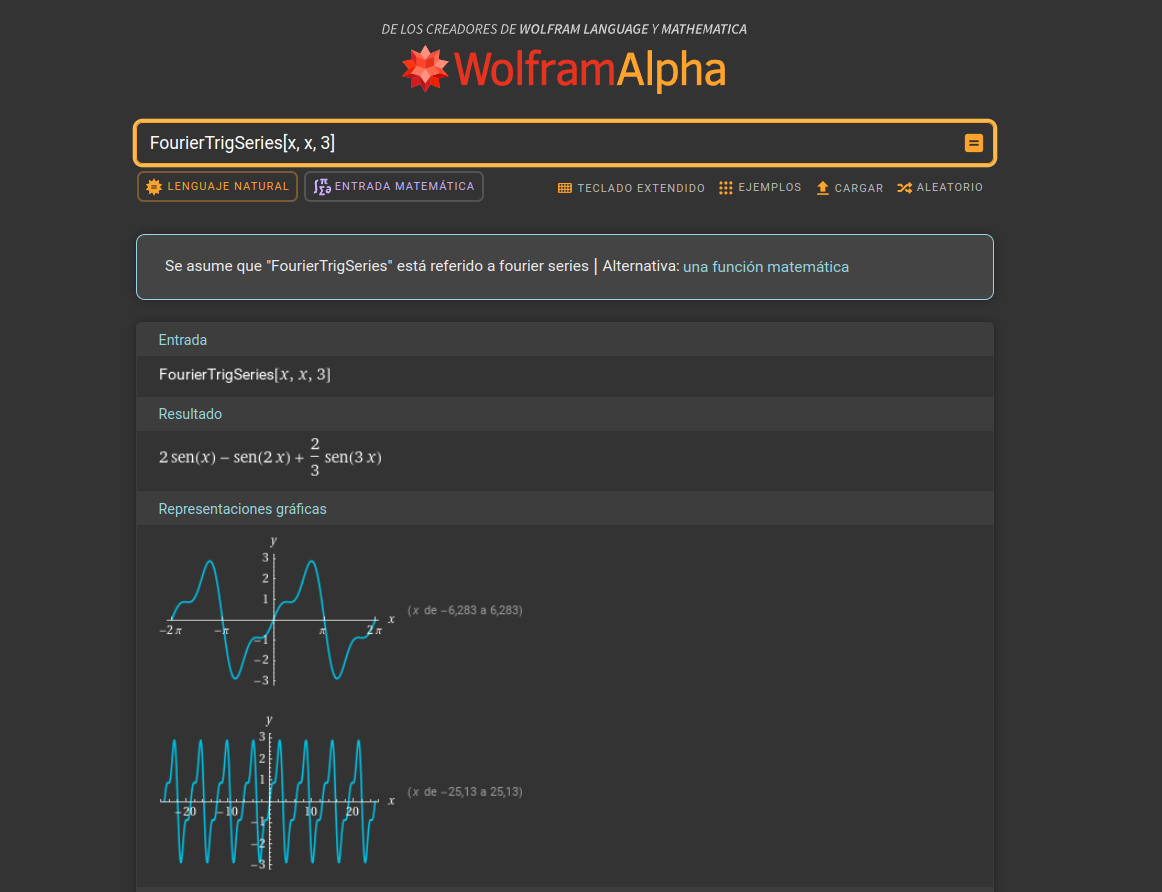
\includegraphics[width=1\textwidth]{img/chapter02/wolfram_trig_series.png}
	\caption{Calculo de una serie trigonométrica de Fourier en WolframAlpha}
	\label{fig:wolfram-trig-series}  % Etiqueta para la figura
\end{figure}
Ahora usaremos la función de \texttt{FourierSeries(exp, t, n)} de WolframAlpha, esta función no permite calcular la serie exponencial compleja de Fourier de la función \texttt{exp} respecto a la variable \texttt{t} obteniendo la serie hasta el término \texttt{n}.
\begin{figure}[H]
	\centering
	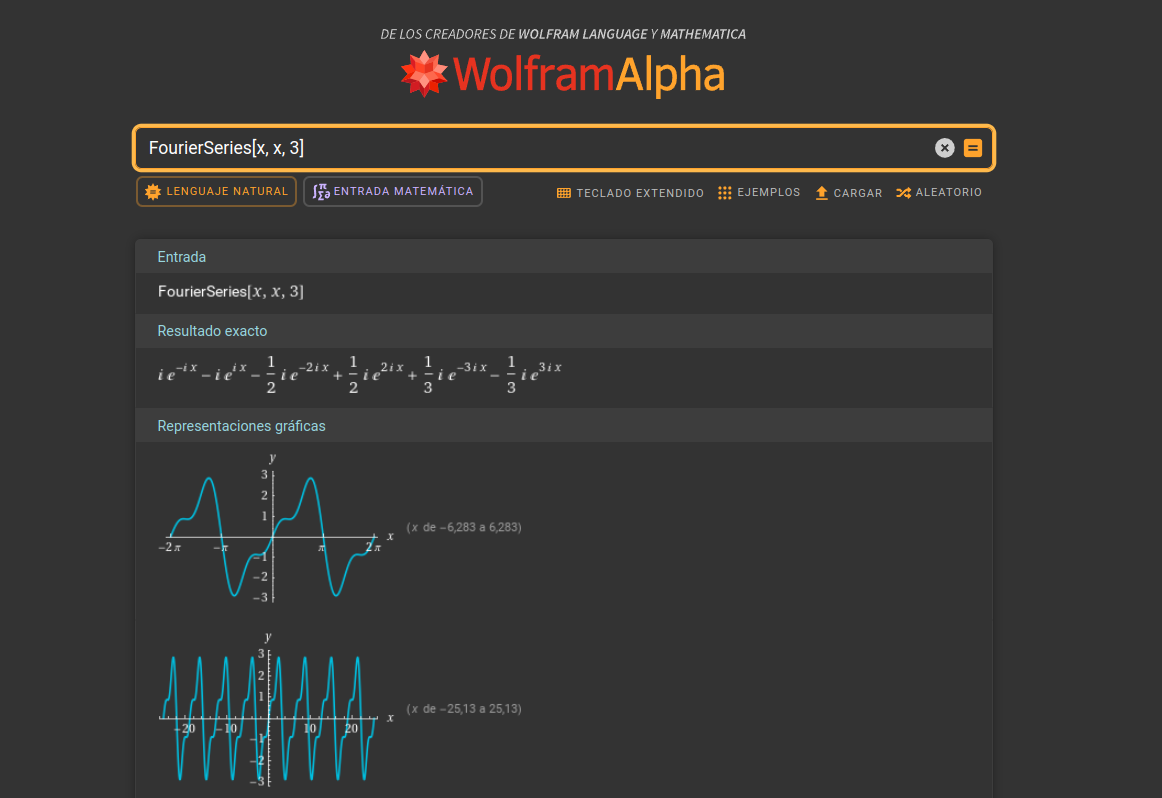
\includegraphics[width=1\textwidth]{img/chapter02/wolfram_complex_series.png}
	\caption{Calculo de una serie trigonométrica de Fourier en WolframAlpha}
	\label{fig:wolfram-exp-series}  % Etiqueta para la figura
\end{figure}
Wolfram nos devuelve la expansión de cada serie en su forma mas reducida, ademas de dos pequeñas gráficas de nuestra aproximación vista desde  no nos devuelve los coeficientes de la serie ni tampoco su expresión final en notación de serie.

\subsection{Symbolab}
Symbolab es una calculadora digital que ayuda a resolver problemas matemáticos, como ecuaciones, álgebra o cálculo. Se trata de una herramienta que cuyo principal proposito es ayudar a sus usuarios a aprender matemáticas, ya que ofrece resoluciones paso a paso y conocimientos impulsados por inteligencia artificial. ~\cite{symbolabDocs}. 
\begin{figure}[H]
	\centering
	
\includegraphics[width=0.3\textwidth]{img/chapter02/logo_symbolab.png}
	\caption[Logotipo de Symbolab.]{Logotipo de Symbolab. \textit{Fuente: ~\cite{symbolabDocs}}}
	\label{fig:logo-symbolab}  % Etiqueta para la figura
\end{figure}
Symbolab se centra en la enseñanza de procedimientos matemáticos mediante explicaciones detalladas. Su interfaz es especialmente útil para estudiantes, ya que presenta guías paso a paso para temas como derivadas, integrales y ecuaciones algebraicas complejas, lo cual es ideal para el aprendizaje autodidacta. Este cuenta con una función para resolver series de Fourier en su forma trigonométrica denominada \texttt{fourier series (f), [-L, L]} ~\cite{symbolabDocs} en donde \texttt{f} es una función definida en el intervalo de \texttt{[-L, L]}. A pesar de contar con funciones para definir funciones matemáticas a trozos y funciones para hacer gráficas, no es posible unificarlas en la misma aplicación, ademas de no contar con funciones para otras series de Fourier como extensiones de medio rango o exponencial compleja, pero, al igual que en Wolfram Alpha, se pueden calcular individualmente los coeficientes con la función \texttt{integral from a to b of x}~\cite{symbolabDocs}.

\subsubsection{Prueba Symbolab}
Para nuestra siguiente prueba, calcularemos la serie de Fourier trigonométrica de de la función calculada en el \hyperref[app1:trig-coeff]{Apendice A}, para hacerlo usaremos la función \texttt{fourier series (f), [-L, L]} de Symbolab, que nos permite calcular la serie trigonométrica de Fourier de la función \texttt{f} respecto a la variable obteniendo desde el intervalo \texttt{-L} a \texttt{L}.
\begin{figure}[H]
	\centering
	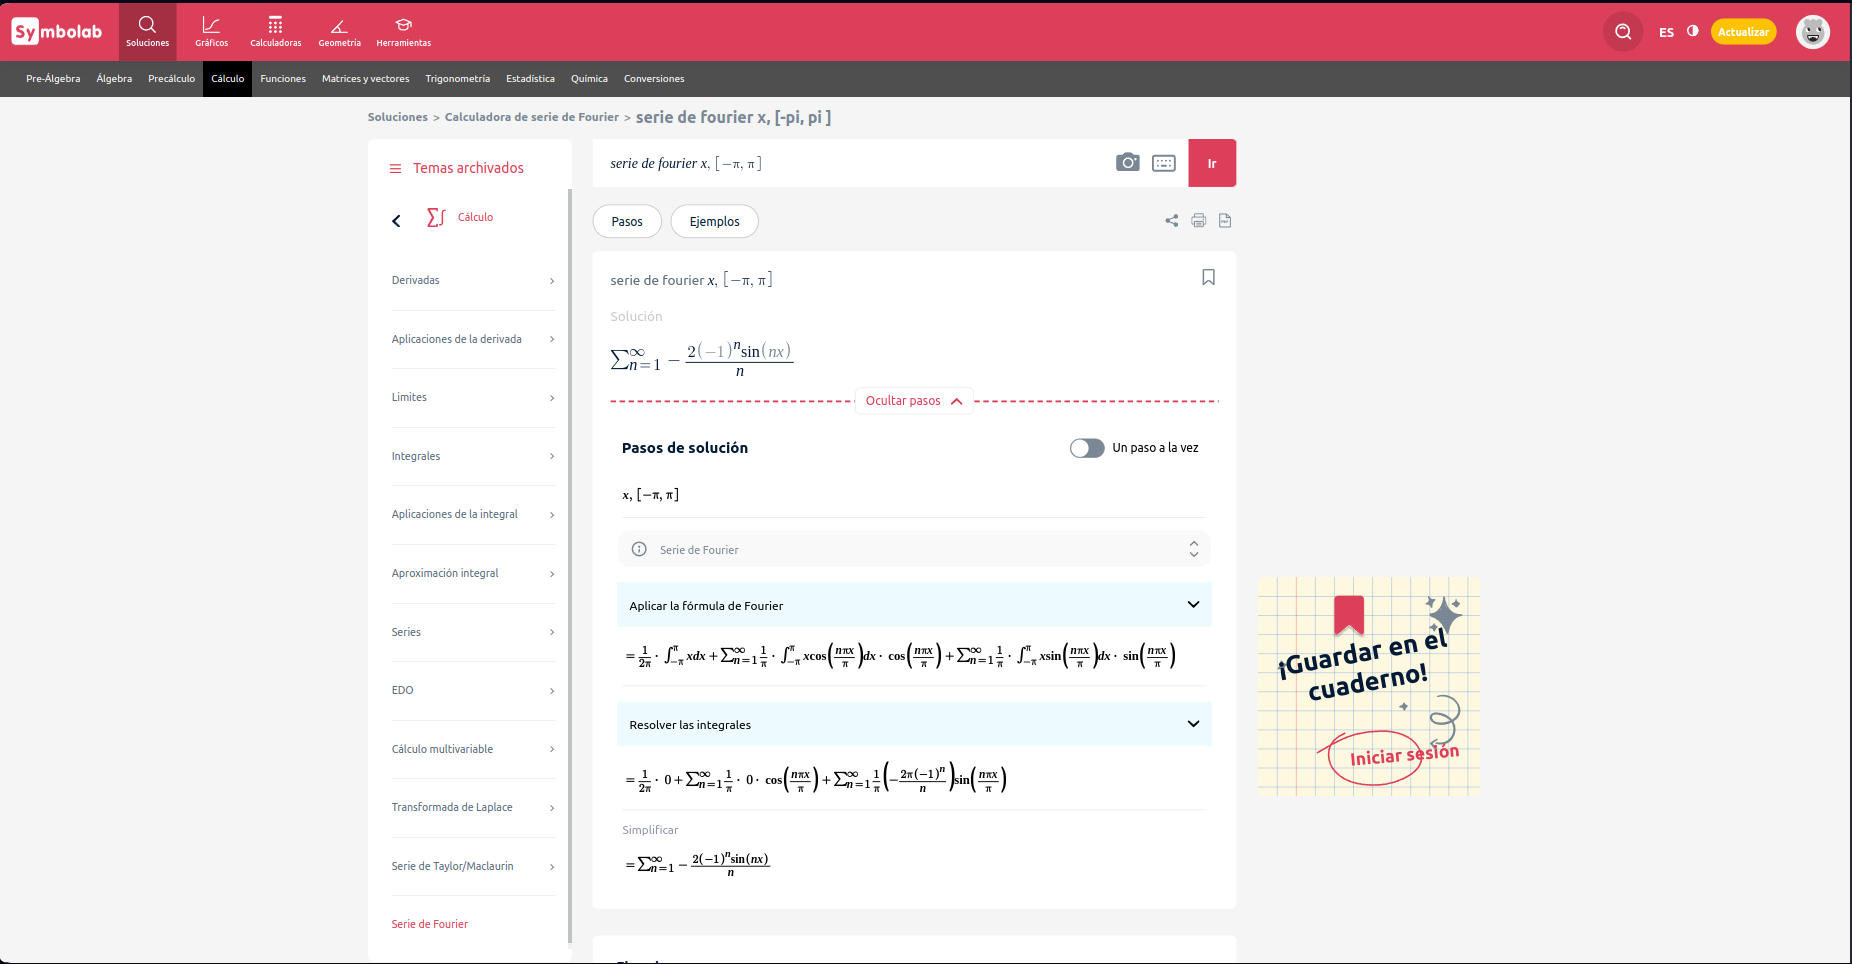
\includegraphics[width=1\textwidth]{img/chapter02/symbolab-trig-series.png}
	\caption{Calculo de una serie trigonométrica de Fourier en Symbolab}
	\label{fig:symbolab-trig-series}  % Etiqueta para la figura
\end{figure}
Symbolab nos dará la expresión en forma de serie, y solo podremos hacerlo para la serie trigonométrica, ademas de que no nos muestra ninguna gráfica.

\subsection{MATLAB} 
MATLAB es un entorno de programación y un lenguaje de alto nivel comercial ampliamente utilizado en ingeniería, física y matemáticas aplicadas para el análisis numérico, la visualización de datos y el desarrollo de algoritmos. Su robusta caja de herramientas, especialmente la \textit{Signal Processing Toolbox} y la \textit{Symbolic Math Toolbox}, facilitan el cálculo y la graficación de series de Fourier  ~\cite{MathWorks2024}.

\begin{figure}[H]
	\centering
	
\includegraphics[width=0.5\textwidth]{img/chapter02/logo_matlab.png}
	\caption[Logotipo de Matlab.]{Logotipo de Matlab. \textit{Fuente: ~\cite{MathWorks2024}}}
	\label{fig:logo-matlab}  % Etiqueta para la figura
\end{figure}

A pesar de que MATLAB cuenta con funciones especiales para el análisis de Fourier como la transformada de Fourier (\texttt{fourier(f)}) o la Transformada rápida de Fourier (\texttt{fft(f)}) no cuenta con funciones especificas para series de Fourier, sin embargo, podemos definir nuestros coeficientes para hacer el gráfico de ambas series.

\subsubsection{Prueba Matlab}
Para la prueba con Matlab, primero ejecutaremos el código en \hyperref[app2:trig-code-matlab]{Apendice B}, que nos graficará la serie de Fourier a partir de sus coeficientes trigonométricos \ref{fig:matlab-trig-series}. 
\begin{figure}[H]
	\centering
	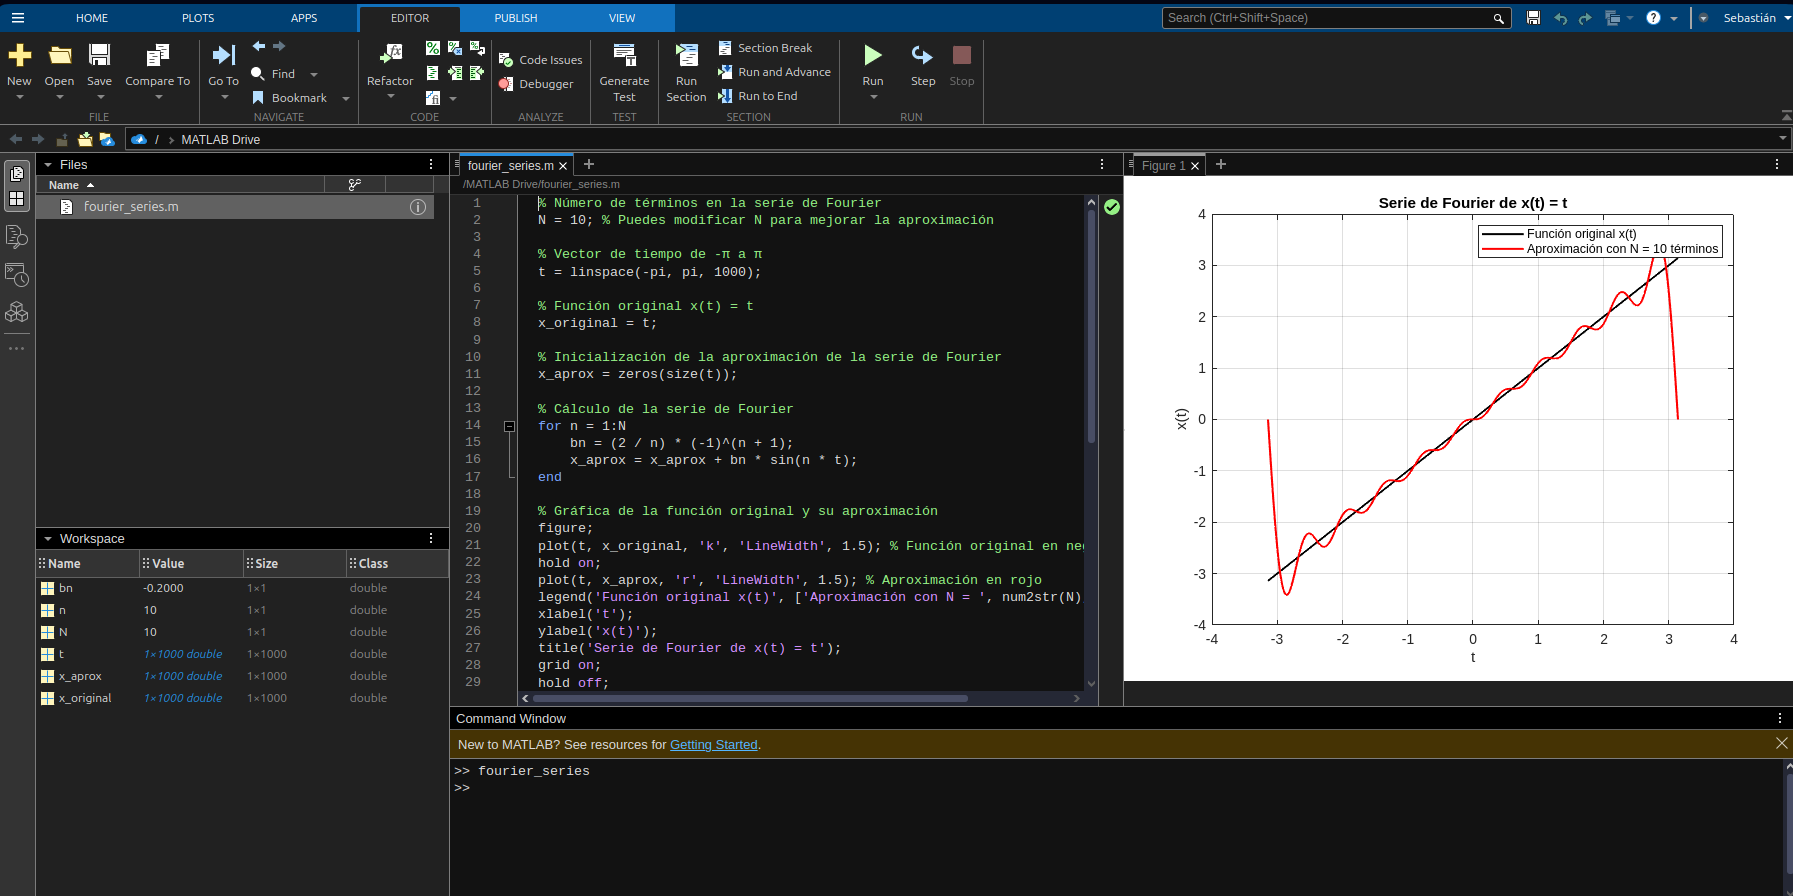
\includegraphics[width=1\textwidth]{img/chapter02/matlab-fourier-trig.png}
	\caption{Graficación de una serie trigonométrica de Fourier en Matlab}
	\label{fig:matlab-trig-series}  % Etiqueta para la figura
\end{figure}
Ahora usamos el código en \hyperref[app2:complex-code-matlab]{Apendice B} para graficar la misma serie pero ahora usando su coefciente complejo \ref{fig:matlab-complex-series}.
\begin{figure}[H]
	\centering
	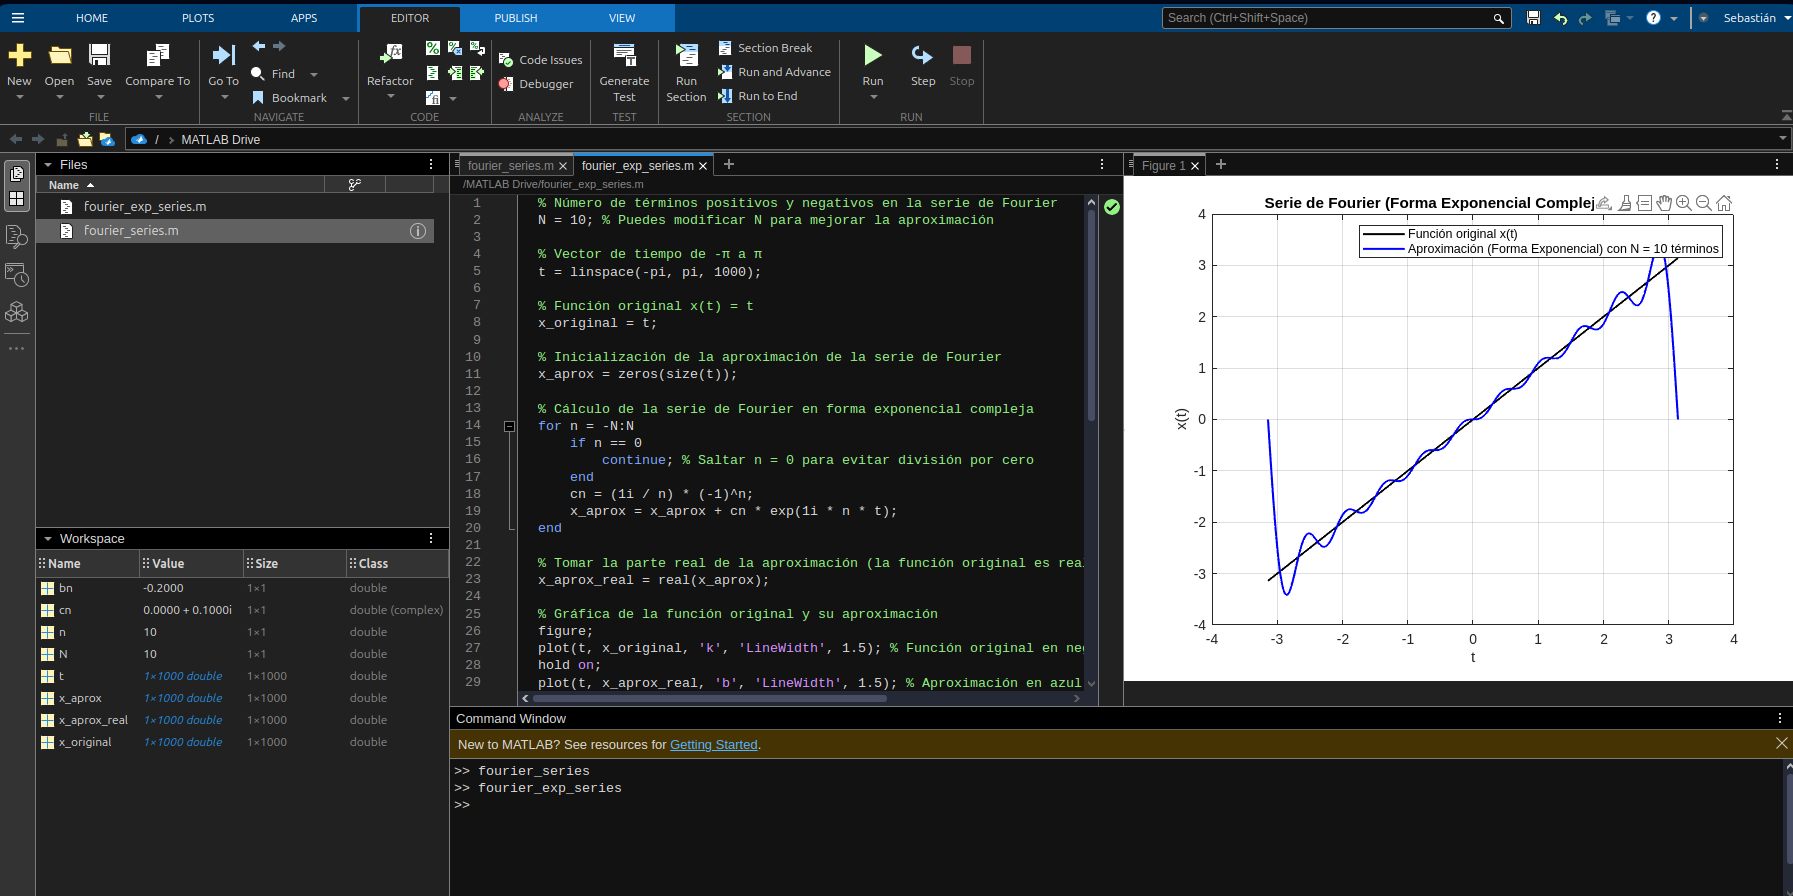
\includegraphics[width=1\textwidth]{img/chapter02/matlab-complex-series.png}
	\caption{Graficación de una serie compleja de Fourier en Matlab}
	\label{fig:matlab-complex-series}  % Etiqueta para la figura
\end{figure}
Matlab es capaz de graficar muy buenas aproximaciones de ambas series en una gráfica que nos brinda cierto nivel de interactividad pero todo dependerá de nuestros cálculos y de que tanto detalle plasmemos en nuestro código para aumentar las funcionalidades

\subsection{Maple}
Maple, desarrollado por Maplesoft, es un Sistema de Álgebra Computacional comercial que permite realizar cálculos matemáticos simbólicos y numéricos, resolver ecuaciones, analizar datos y crear visualizaciones gráficas en 2D y 3D. Maple utiliza el paradigma REPL (Read-Eval-Print Loop), un entorno interactivo donde cada línea de código ingresada es leída, evaluada y su resultado es impreso inmediatamente, facilitando así la experimentación y el desarrollo incremental de cálculos complejos.~\cite{maple2024}.
\begin{figure}[H]
	\centering
	
\includegraphics[width=0.5\textwidth]{img/chapter02/logo_maple.png}
	\caption[Logotipo de Maple.]{Logotipo de Maple. \textit{Fuente: ~\cite{maple2024}}}
	\label{fig:logo-maple}  % Etiqueta para la figura
\end{figure}
Si bien este CAS cuenta con funciones dedicadas al calculo de series de Fourier, estás vienen definidas en paquetes desarrollados por la comunidad de Maplesoft ~\cite{mapleFourier}, así que resulta más eficiente y conveniente usar las funciones de integración (\texttt{int(f, x = a..b)} calcula simbólicamente la integral de \texttt{f}, que depende de la variable \texttt{x} desde el punto \texttt{a} hasta el \texttt{b}) para calcular los coeficientes, y para expandir series (\texttt{seq(m, n = a..b)} en donde \texttt{m} es la función a sumar,sobre la variable \texttt{n} desde el punto \texttt{a} hasta el \texttt{b}) las funciones de expansión, además de poder declarar una función a trozos con la función \texttt{piecewise(cond-1, f-1, cond-2, f-2, ..., cond-n, f-n, f-otherwise)}.

\subsubsection{Prueba Maple}
Para la prueba con Maple, primero ejecutaremos el código en \hyperref[app2:trig-code-maple]{Apendice B}, que, primeramente, calculará los coeficientes de la serie trigonométrica \ref{fig:maple-trig-series}. 
\begin{figure}[H]
	\centering
	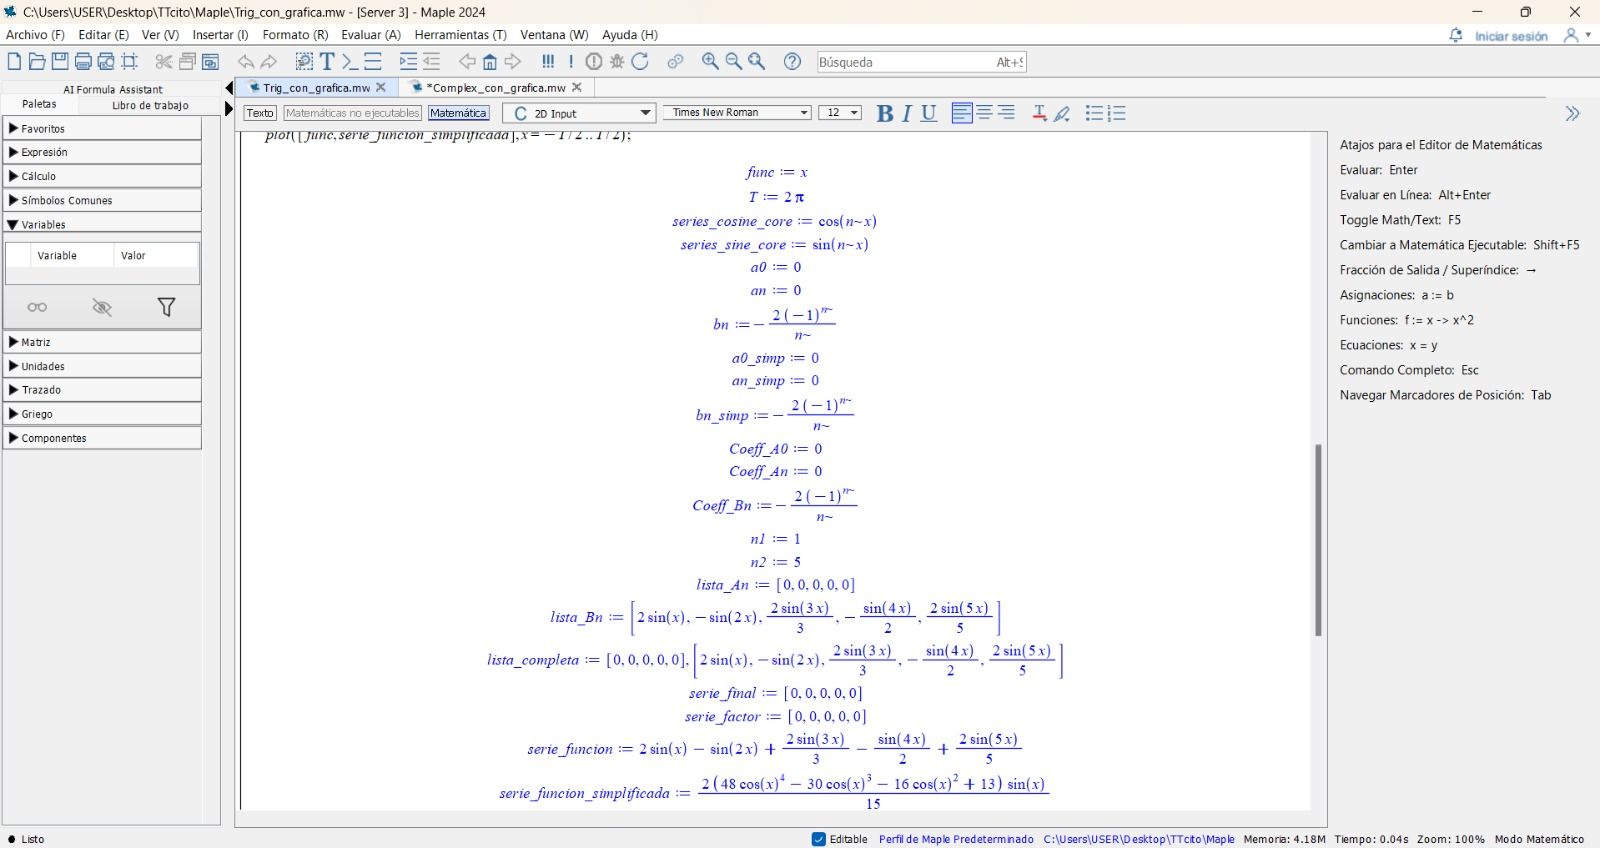
\includegraphics[width=1\textwidth]{img/chapter02/maple-trig-series-coeff.jpeg}
	\caption{Cálculos de coeficientes trigonométricos de Fourier en Maple}
	\label{fig:maple-trig-series}  % Etiqueta para la figura
\end{figure}

Posteriormente, este código nos dará una gráfica estática con los valores que le establecimos \hyperref[app2:trig-code-maple]{Apendice B} \ref{fig:maple-trig-series-graph}. 
\begin{figure}[H]
	\centering
	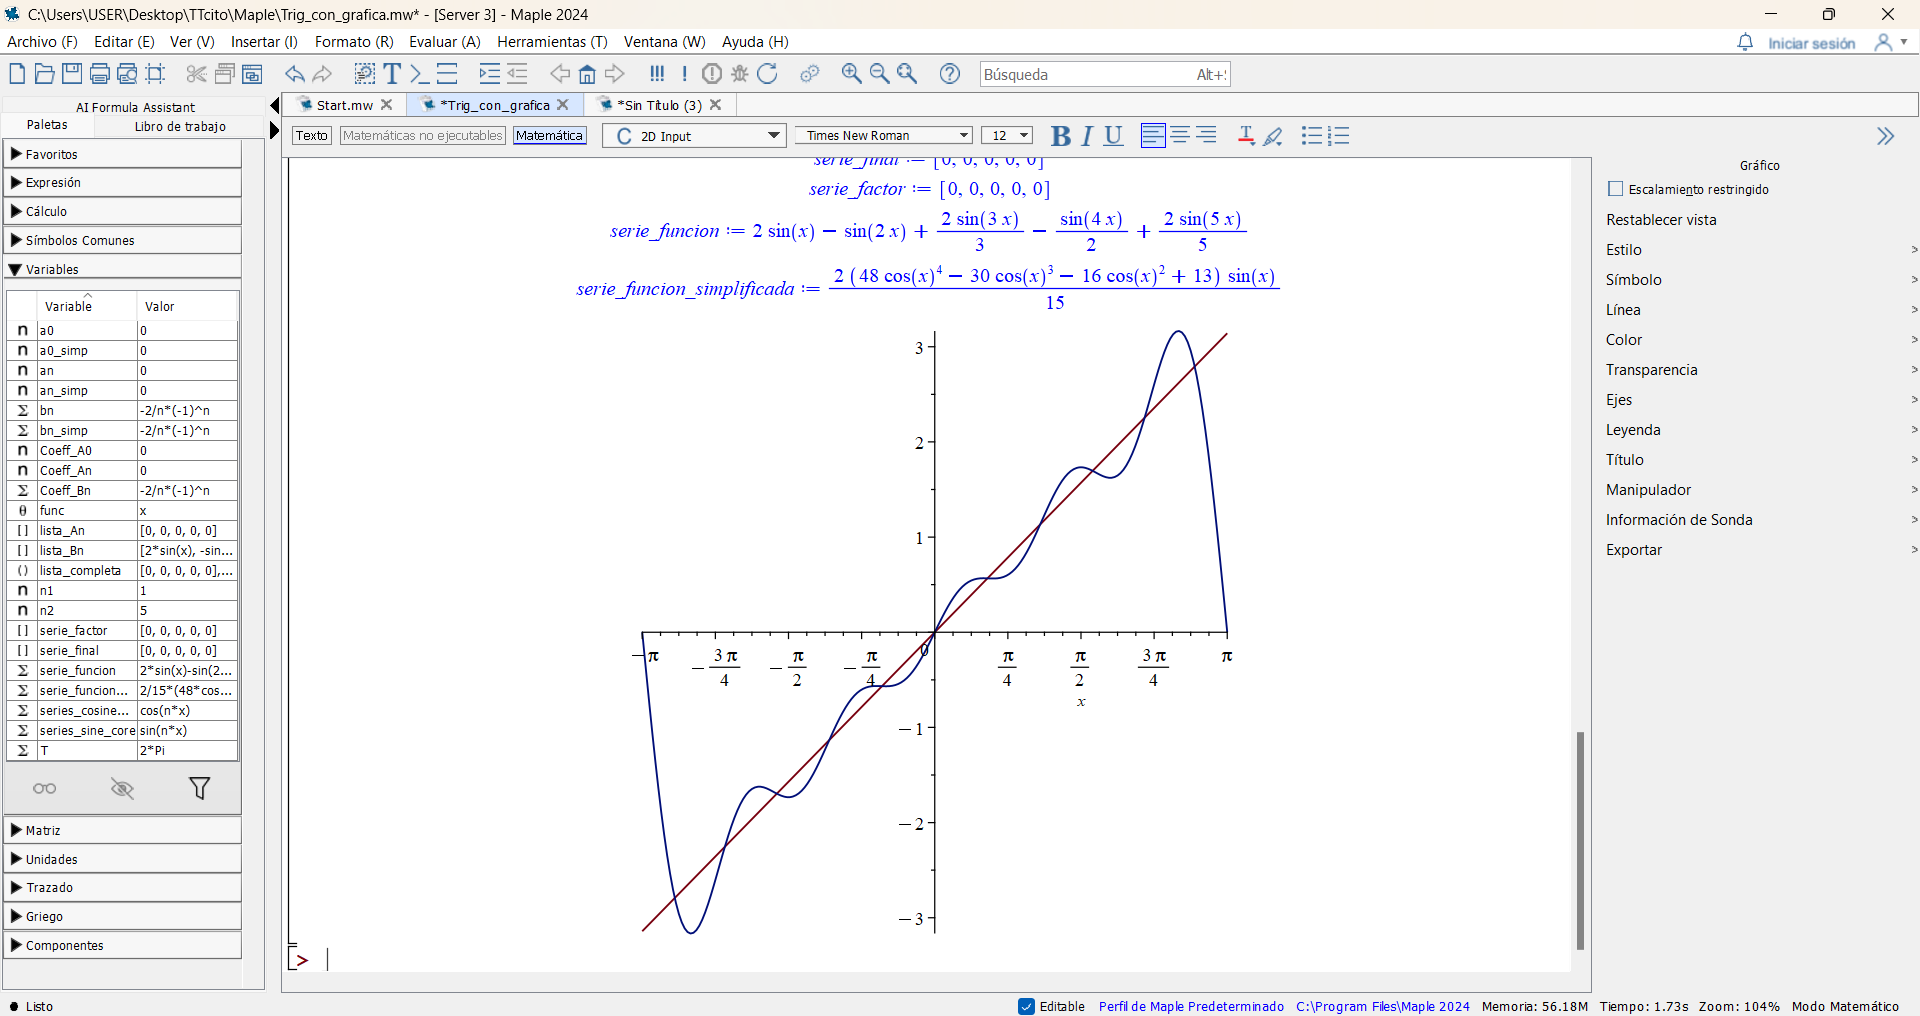
\includegraphics[width=1\textwidth]{img/chapter02/maple-trig-graph.png}
	\caption{Grafica de la serie de Fourier trigonométrica en Maple}
	\label{fig:maple-trig-series-graph}  % Etiqueta para la figura
\end{figure}
Podemos ver que puede resolver la serie trigonométrica sin problema alguno, ahora veamos la misma función pero desarrollada en una serie exponencial compleja  \hyperref[app2:complex-code-maple]{Apendice B}.
\begin{figure}[H]
	\centering
	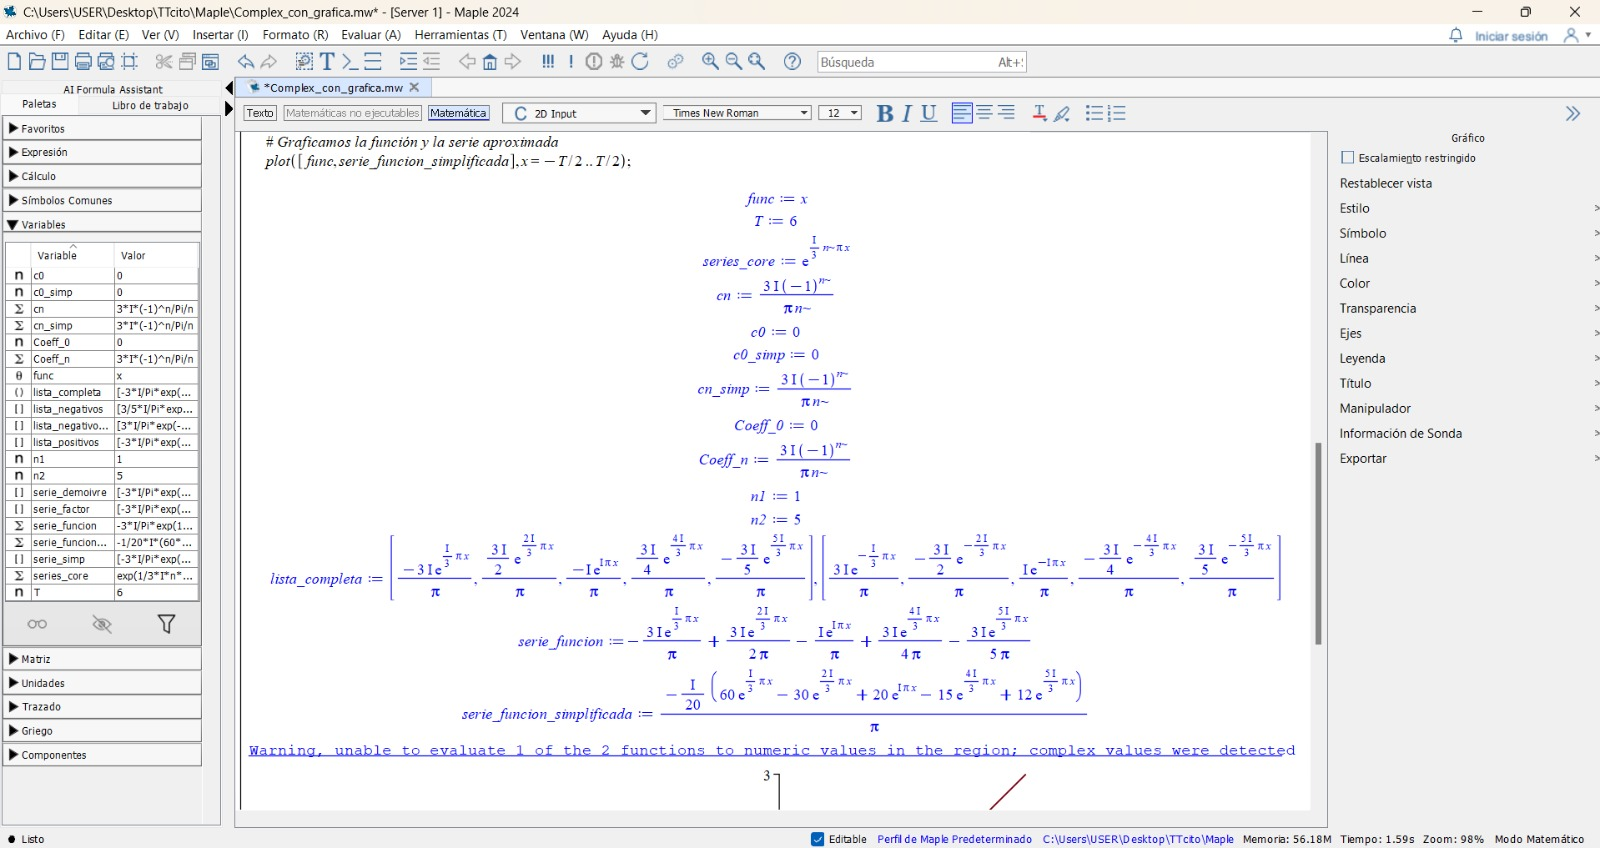
\includegraphics[width=1\textwidth]{img/chapter02/maple-complex-series-coeff.jpeg}
	\caption{Cálculo del coeficiente complejo de Fourier en Maple}
	\label{fig:maple-complex-series}  % Etiqueta para la figura
\end{figure}

De igual modo, este código nos dará una gráfica estática con los valores que le establecimos \hyperref[app2:trig-code-maple]{Apendice B} \ref{fig:maple-trig-series-graph}. 
\begin{figure}[H]
	\centering
	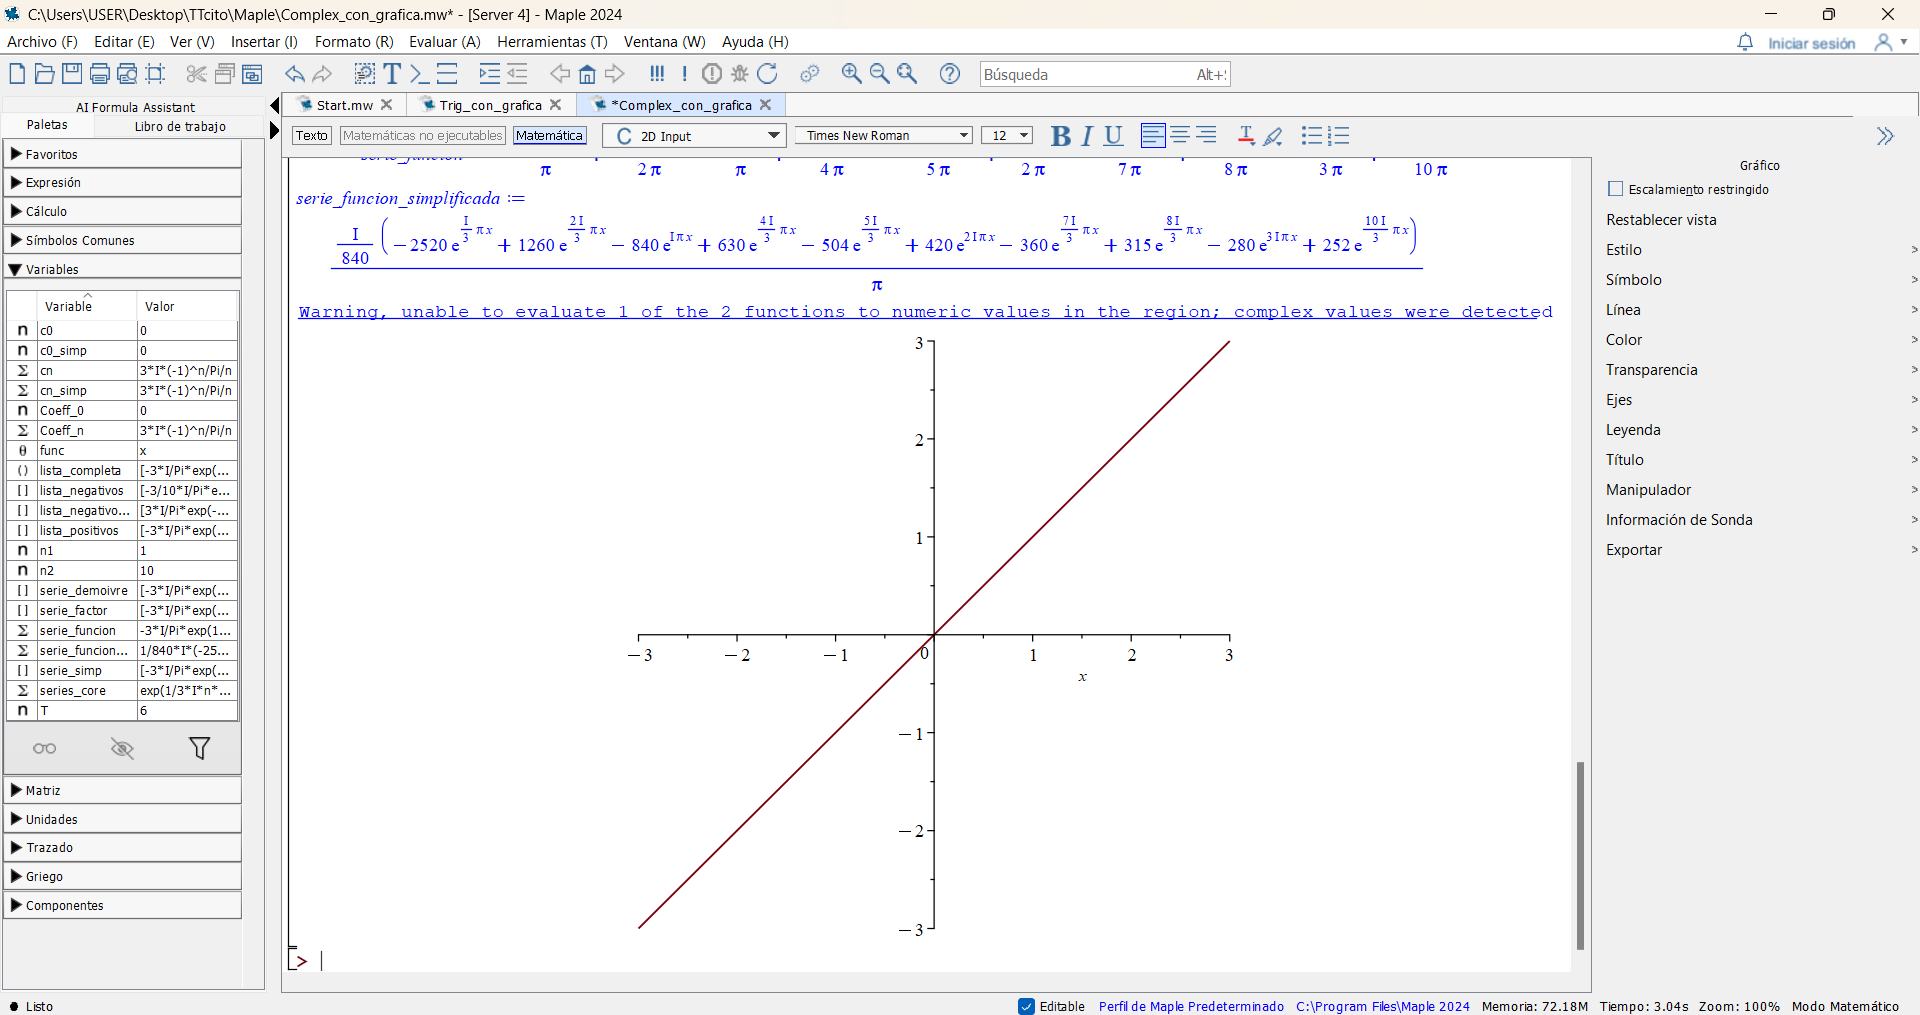
\includegraphics[width=1\textwidth]{img/chapter02/maple-complex-graph.png}
	\caption{Grafica de la serie de Fourier compleja en Maple}
	\label{fig:maple-complex-series-graph}  % Etiqueta para la figura
\end{figure}
El detalle está en que no hay forma de graficar nuestra función serie compleja ya que no puede hacer las cancelaciones entre los números imaginarios al expandir la serie, por lo tanto, la función la mantiene en el dominio de los números complejos y no la puede graficar en el plano real. Una alternativa sería graficar la serie trigonométrica que obtuvimos en \ref{fig:maple-trig-series-graph} ya que son equivalentes.

\subsection{Maxima}
Maxima es un Sistema de Álgebra Computacional de código abierto y gratuito, derivado del sistema Macsyma desarrollado en la década de 1980. Permite realizar cálculos simbólicos y numéricos avanzados, como derivadas, integrales, simplificación de expresiones algebraicas, resolución de ecuaciones y generación de gráficos en 2D y 3D. Maxima emplea el paradigma REPL (Read-Eval-Print Loop), proporcionando un entorno interactivo donde cada comando ingresado se procesa de inmediato, lo que facilita la verificación y corrección rápida de cálculos ~\cite{MaximaSourgeforce}. 
\begin{figure}[H]
	\centering
	
\includegraphics[width=0.5\textwidth]{img/chapter02/logo_maxima.png}
	\caption[Logotipo de Maxima.]{Logotipo de Maxima. \textit{Fuente: ~\cite{MaximaSourgeforce}}}
	\label{fig:logo-maxima}  % Etiqueta para la figura
\end{figure}
Si bien, este CAS al igual que Maple, cuenta con módulo que importa funciones especiales para el análisis de Fourier, este si es propio de Maxima. Sin embargo, igual que en Maple, resulta más practico trabajar con las funciones propias de Maxima para integrar (\texttt{integrate (expr, x, a, b)} Calcula simbólicamente la integral de \texttt{expr} con límites en \texttt{a} y \texttt{b} ) así como su función para expandir una función en serie (\texttt{makelist(expr, i, i\_min, i\_max, step)} Genera una lista evaluando \texttt{expr} para cada valor de \texttt{i} desde \texttt{i\_min} hasta \texttt{i\_max}, incrementando \texttt{i} en \texttt{step} en cada iteración). 

\subsubsection{Prueba Maxima}
Para la prueba con Maxima, ejecutaremos el código en \hyperref[app2:trig-code-maxima]{Apendice B}, que primero calculará los coeficientes de la serie trigonométrica \ref{fig:maple-trig-series}. 
\begin{figure}[H]
	\centering
	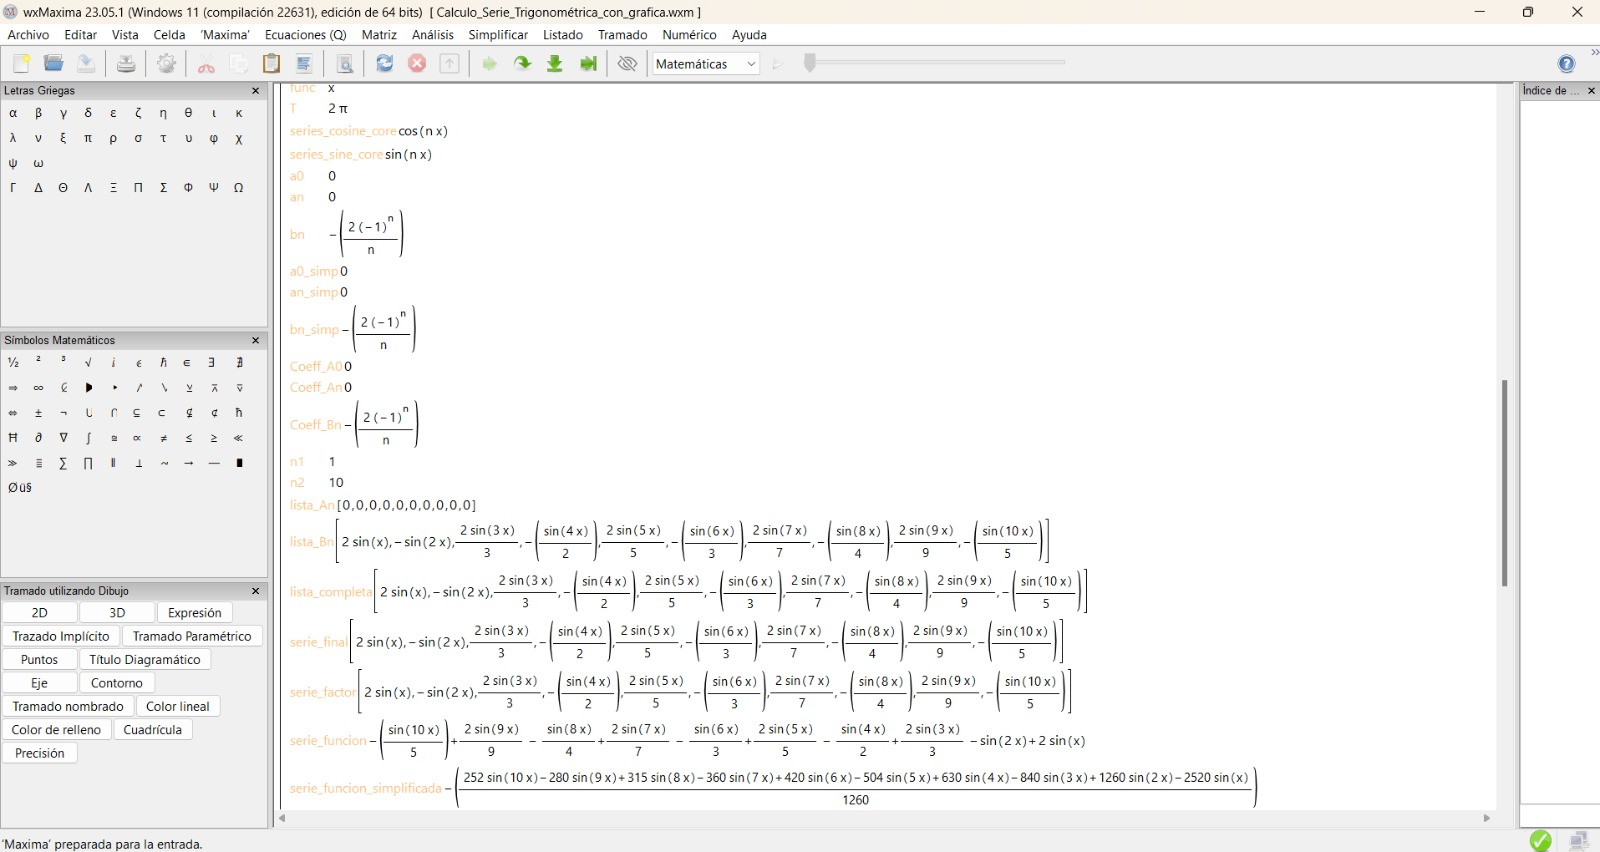
\includegraphics[width=1\textwidth]{img/chapter02/maxima-trig-series-coeff.jpeg}
	\caption{Cálculos de coeficientes trigonométricos de Fourier en Maxima}
	\label{fig:maxima-trig-series}  % Etiqueta para la figura
\end{figure}
Posteriormente, este código nos dará una gráfica dinámica con los valores que le establecimos.
\begin{figure}[H]
	\centering
	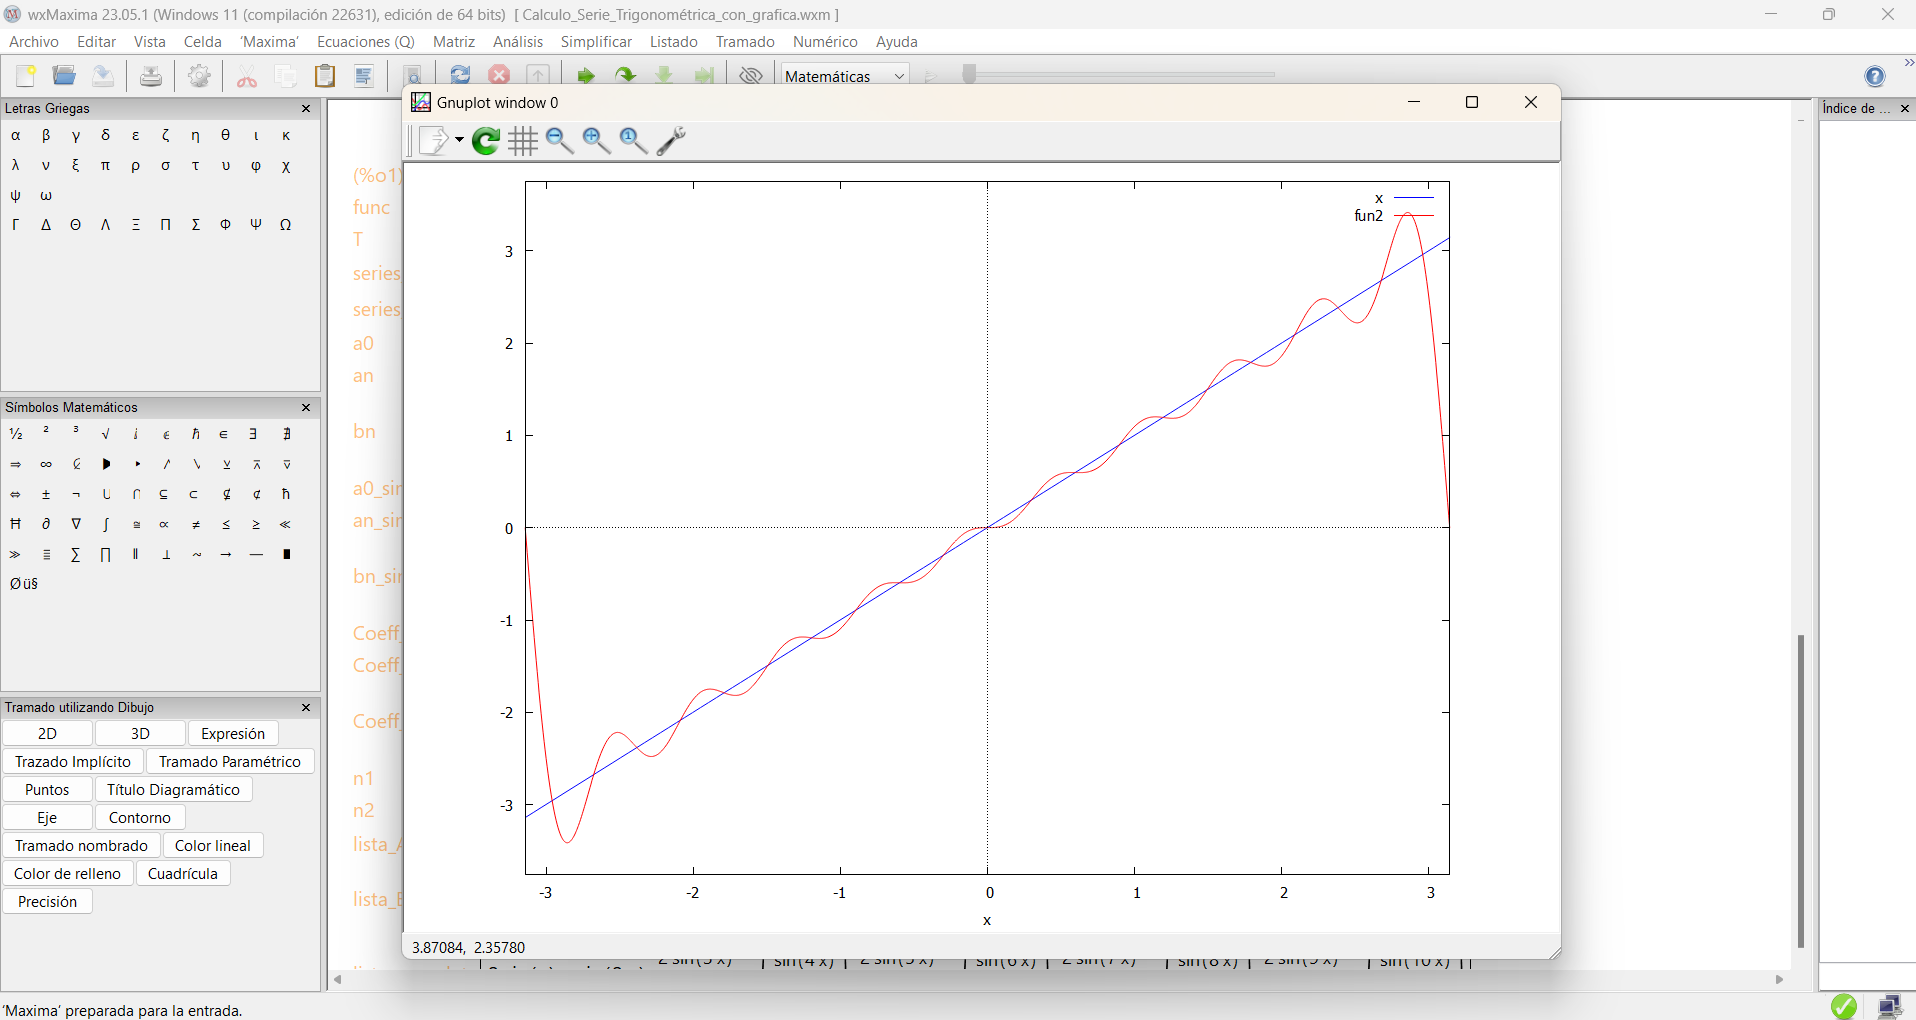
\includegraphics[width=1\textwidth]{img/chapter02/maxima-trig-series-graph.png}
	\caption{Grafica de la serie de Fourier trigonométrica en Maxima}
	\label{fig:maxima-trig-series-graph}  % Etiqueta para la figura
\end{figure}

Podemos ver que sin problema alguno se construye la gráfica, ahora, probemos haciendo el problema de la misma función pero para la serie compleja  \hyperref[app2:complex-code-maxima]{Apendice B}. 

\begin{figure}[H]
	\centering
	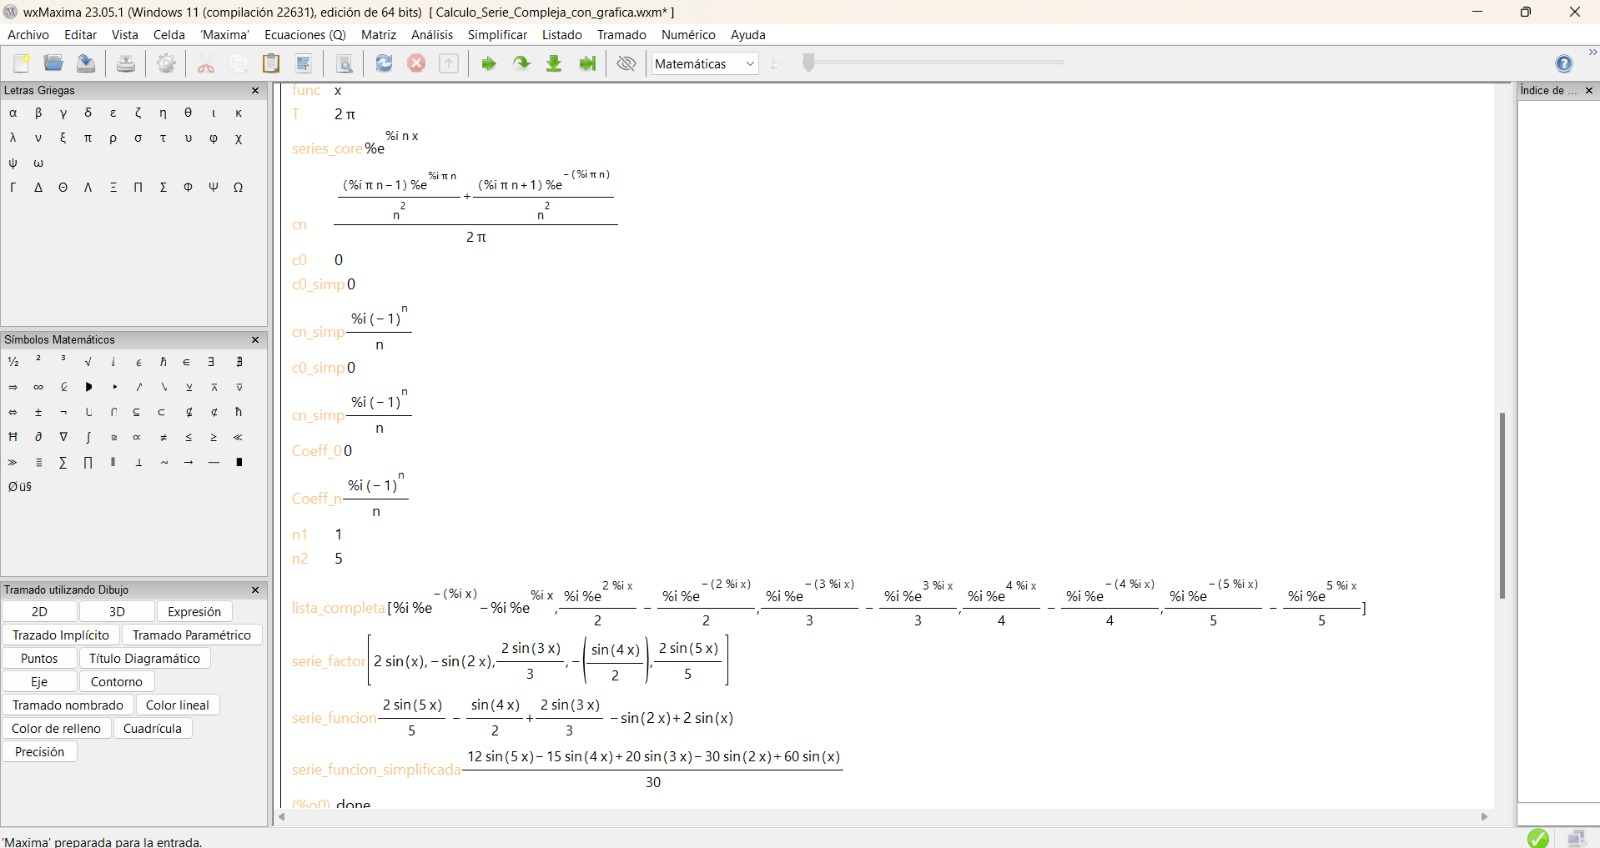
\includegraphics[width=1\textwidth]{img/chapter02/maxima-complex-series-coeff.jpeg}
	\caption{Cálculos de coeficientes compleja de Fourier en Maxima}
	\label{fig:maxima-complex-series}  % Etiqueta para la figura
\end{figure}
De igual modo, este código nos dará una gráfica dinámica con los valores que le establecimos.
\begin{figure}[H]
	\centering
	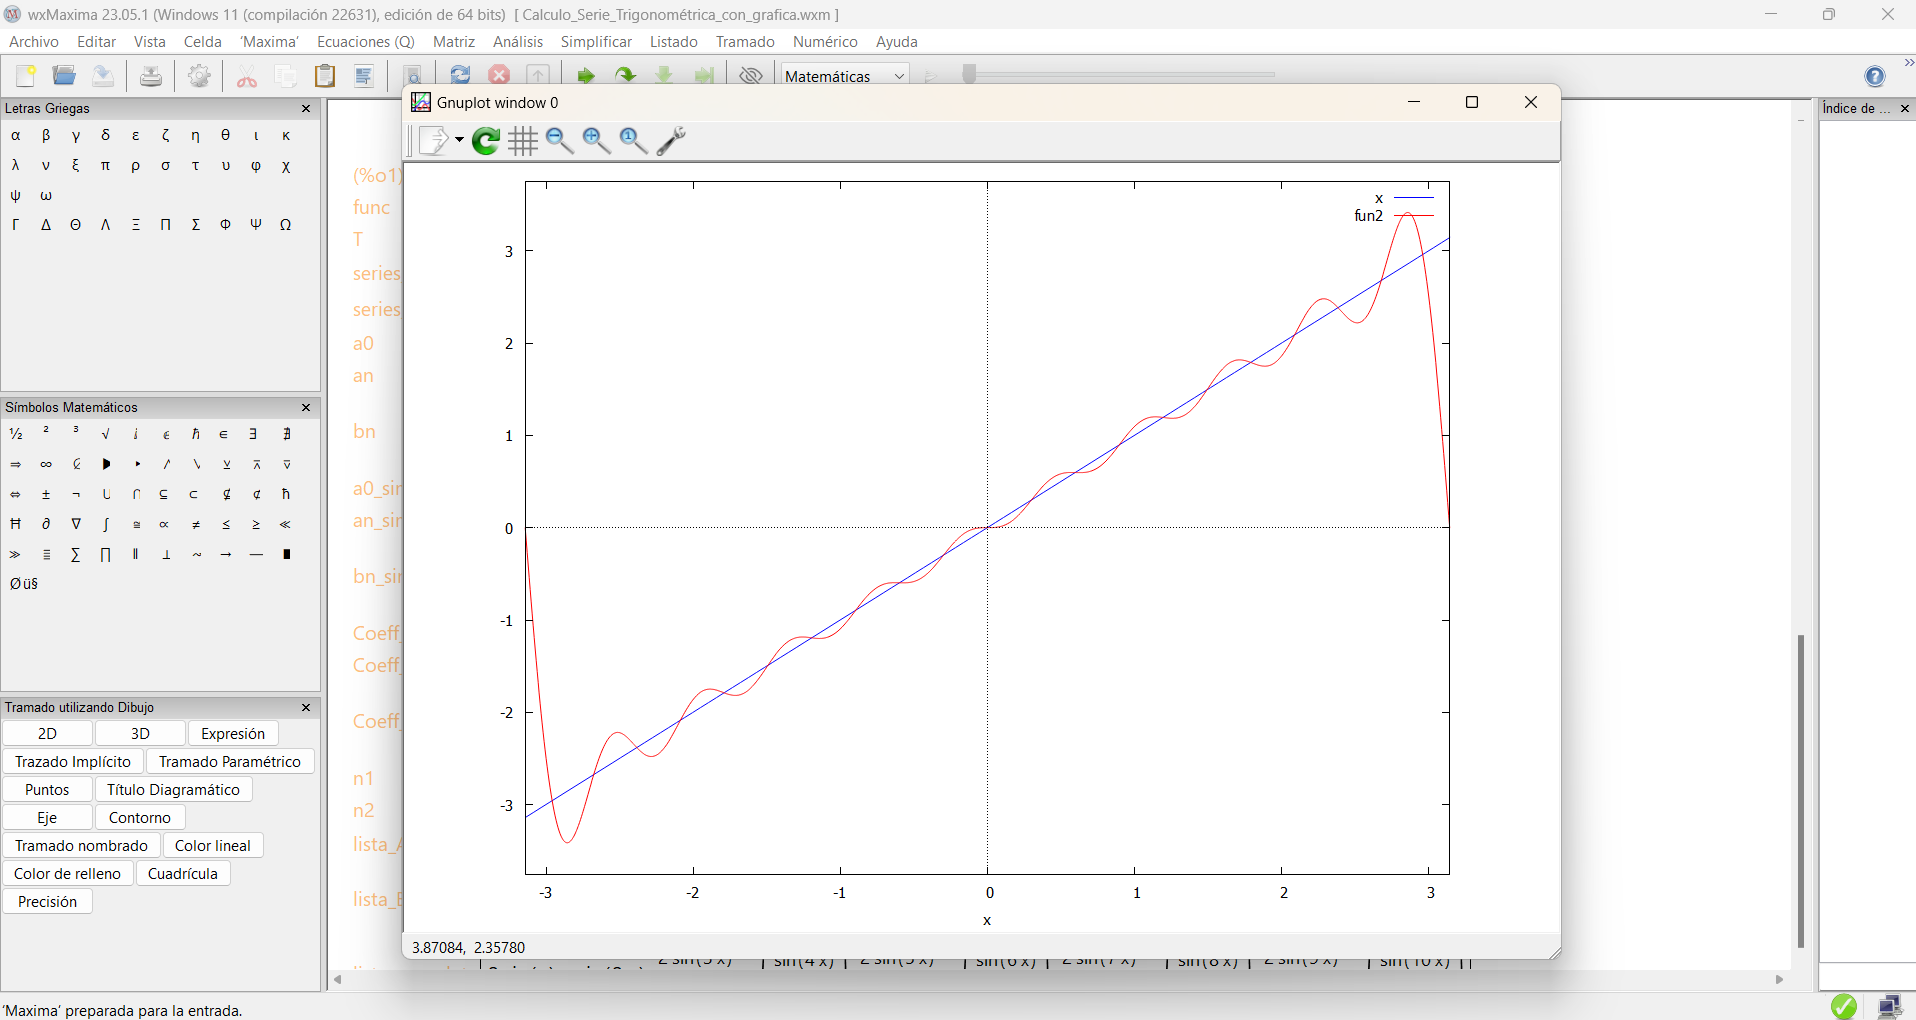
\includegraphics[width=1\textwidth]{img/chapter02/maxima-trig-series-graph.png}
	\caption{Grafica de la serie de Fourier compleja en Maxima}
	\label{fig:maxima-complex-series-graph}  % Etiqueta para la figura
\end{figure}
Podemos observar que sin problemas podemos hacer el gráfico ya que la función \texttt{demoivre()} se encarga de separar la parte real e imaginaria y con esto, hacer la gráfica equivalente.
A pesar de que Maxima no cuenta con una función para declarar funciones a trozos, podemos calcular las integrales por separado o usar matrices (\texttt{matrix (fila\_1, ..., fila\_n)}), pero esto se verá más adelante. 
\subsection{Geogebra / Desmos}
GeoGebra y Desmos son dos herramientas educativas digitales, gratuitas y de código abierto, utilizadas para la enseñanza y el aprendizaje de las matemáticas. Ambas permiten a los usuarios graficar funciones, trabajar conceptos algebraicos y geométricos de manera interactiva, facilitando la visualización y comprensión de diversos temas matemáticos. Estas presentan algunas diferencias: GeoGebra ofrece una suite más completa que incluye módulos para álgebra, geometría, cálculo y estadística, lo que la hace especialmente útil para crear construcciones geométricas dinámicas y realizar análisis más complejos ~\cite{GeoGebra2024}. Por otro lado, Desmos se destaca por su interfaz intuitiva y facilidad de uso, enfocándose principalmente en la gráfica de funciones y proporcionando herramientas sencillas para crear visualizaciones rápidas y efectivas, lo que la hace ideal para estudiantes y educadores que buscan una plataforma accesible y potente para la enseñanza de conceptos fundamentales ~\cite{Desmos2024}.

\begin{figure}[H]
	\centering
	\begin{minipage}{0.4\textwidth}
		\centering
		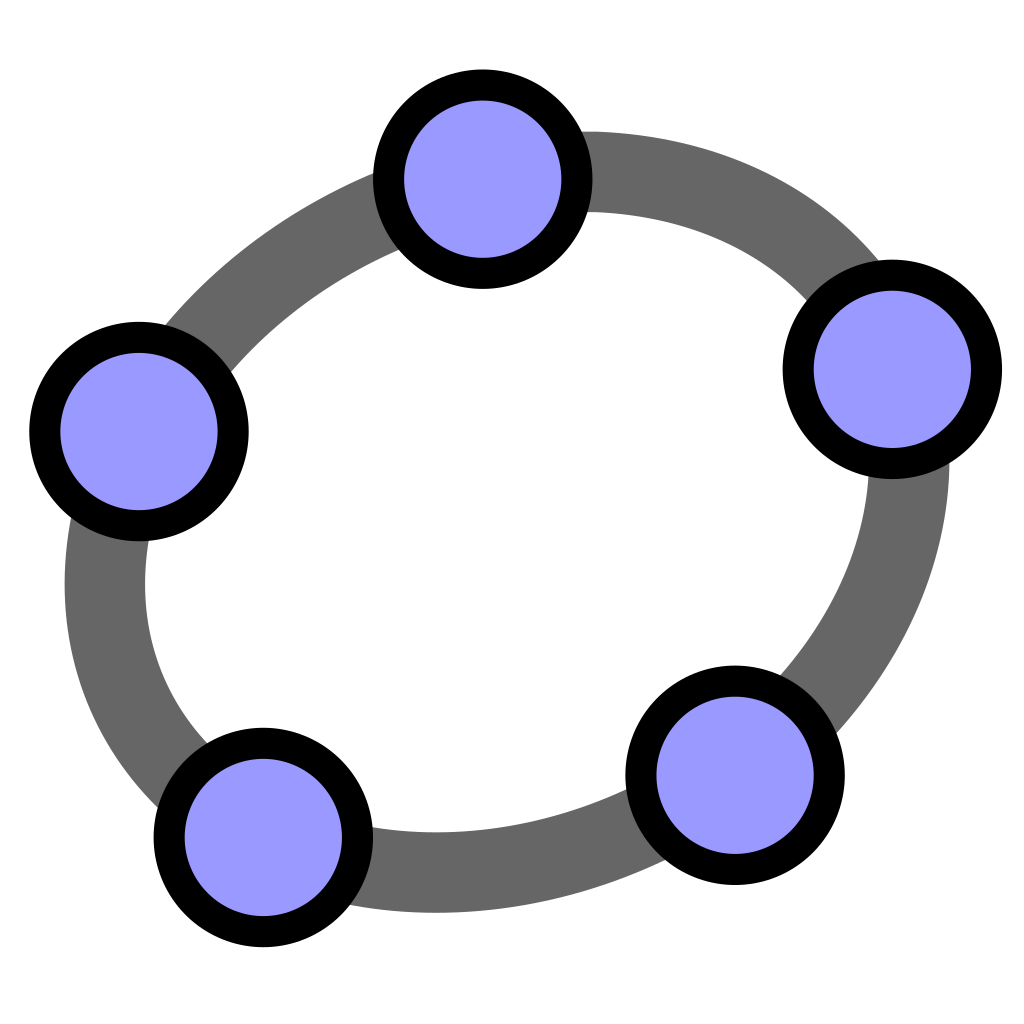
\includegraphics[width=\textwidth]{img/chapter02/logo_geogebra.png}
		\caption[Logotipo de Geogebra.]{Logotipo de Geogebra. \textit{Fuente: ~\cite{wolframMatemathica}}}
		\label{fig:logo-geogebra}
	\end{minipage}%
	\hfill % Añade un espacio entre las imágenes
	\begin{minipage}{0.6\textwidth}
		\centering
		
\includegraphics[width=\textwidth]{img/chapter02/logo_desmos.jpg} % Cambia "otro_logo.jpg" por el nombre de tu segunda imagen
		\caption[Logotipo de Desmos.]{Logotipo de Desmos. \textit{Fuente: ~\cite{Desmos2024}}}
		\label{fig:logo-desmos}
	\end{minipage}
\end{figure}

Si bien, no tienen funciones especificas para el análisis de Fourier, ambas pueden hacer las gráficas de sumas correspondientes a los coeficientes. A continuación mostraremos la gráfica de la serie de Fourier de \ref{app1:trig-coeff} con ambas herramientas.

\subsubsection{Prueba Geogebra}
Para la prueba con Geogebra, crearemos un slider desde 1 hasta el valor que querramos con la única condición de que este de saltos de 1 en 1, es decir, sea un slider de números enteros, también usamos la función de \texttt{Suma(Expresión, Variable, Valor Inicial, Valor Final)} en donde \texttt{Expresión} será la función de la serie, \texttt{Variable} es el n-ésimo termino en la serie, \texttt{Valor Inicial} será 1 y   \texttt{Valor Final} será el valor que toma el slider.
\begin{figure}[H]
	\centering
	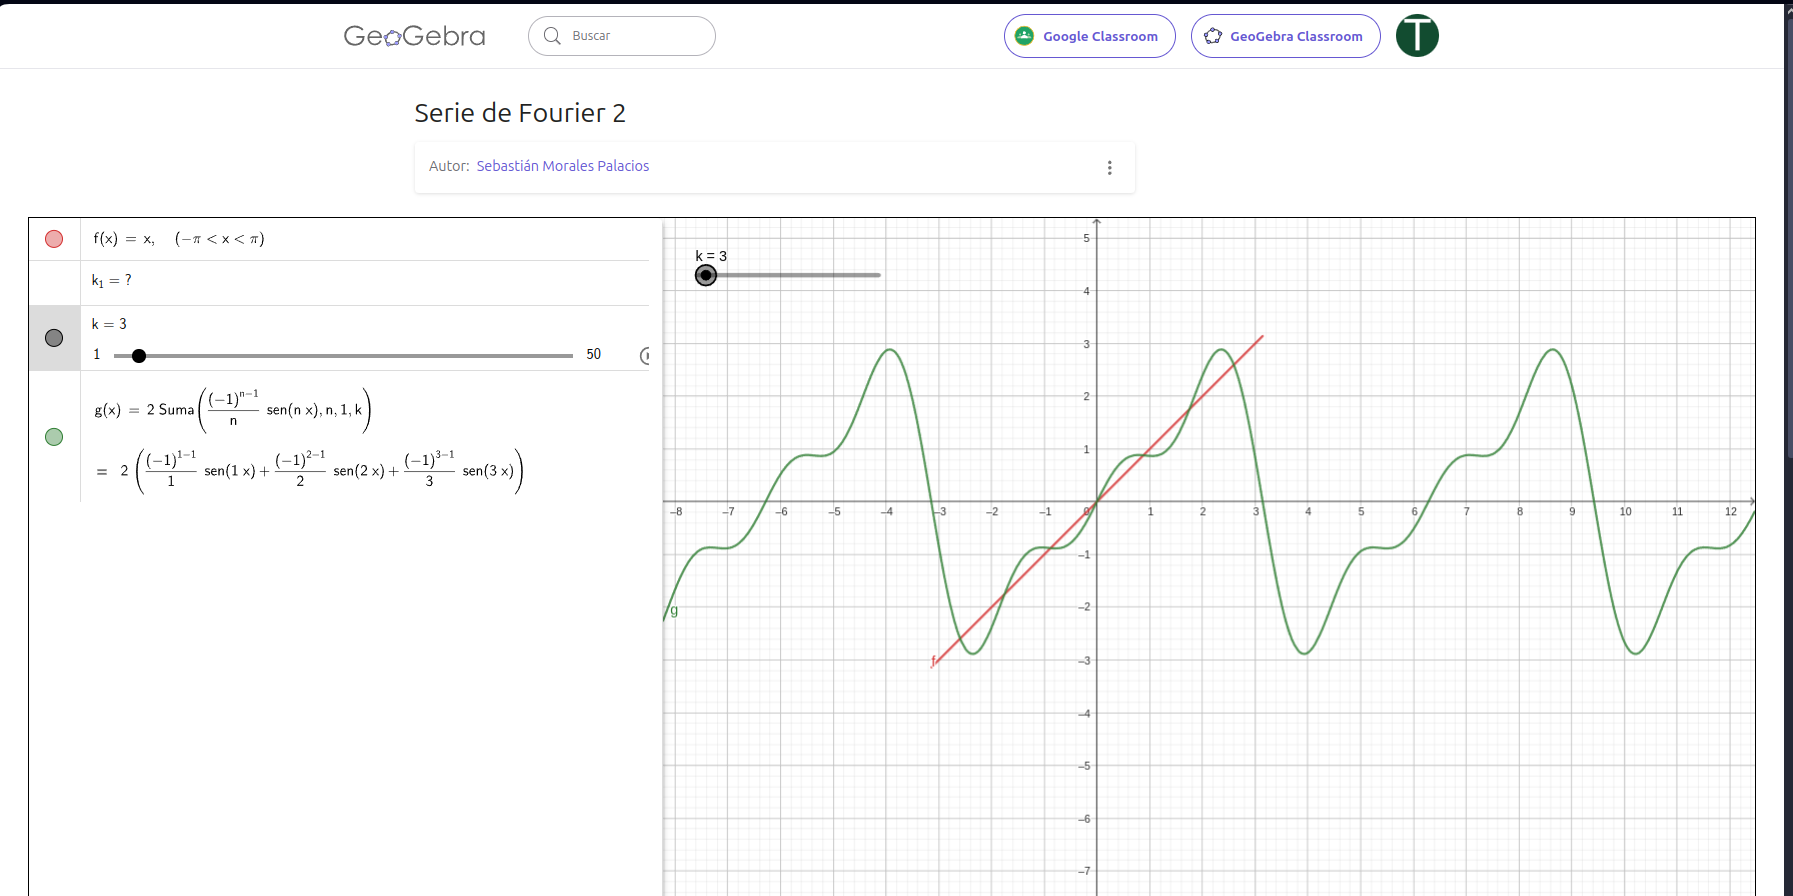
\includegraphics[width=1\textwidth]{img/chapter02/geogebra-trig-series.png}
	\caption{Gráfica de la serie trigonométrica de Fourier en Geogebra}
	\label{fig:geogebra-trig-series}  % Etiqueta para la figura
\end{figure}
Geogebra nos dará una gráfica completamente dinámica pero será un tanto pesada, ya que al añadir más de 5 términos la página comenzará a tener problemas con el dinamismo.

\subsubsection{Prueba Desmos}
Para Desmos será algo más sencillo que en Geogebra, ya que solo tendremos que computar la expresión de la serie sin definir funciones, al terminar de computar la serie nos generará en automático el slider, solo 
\begin{figure}[H]
	\centering
	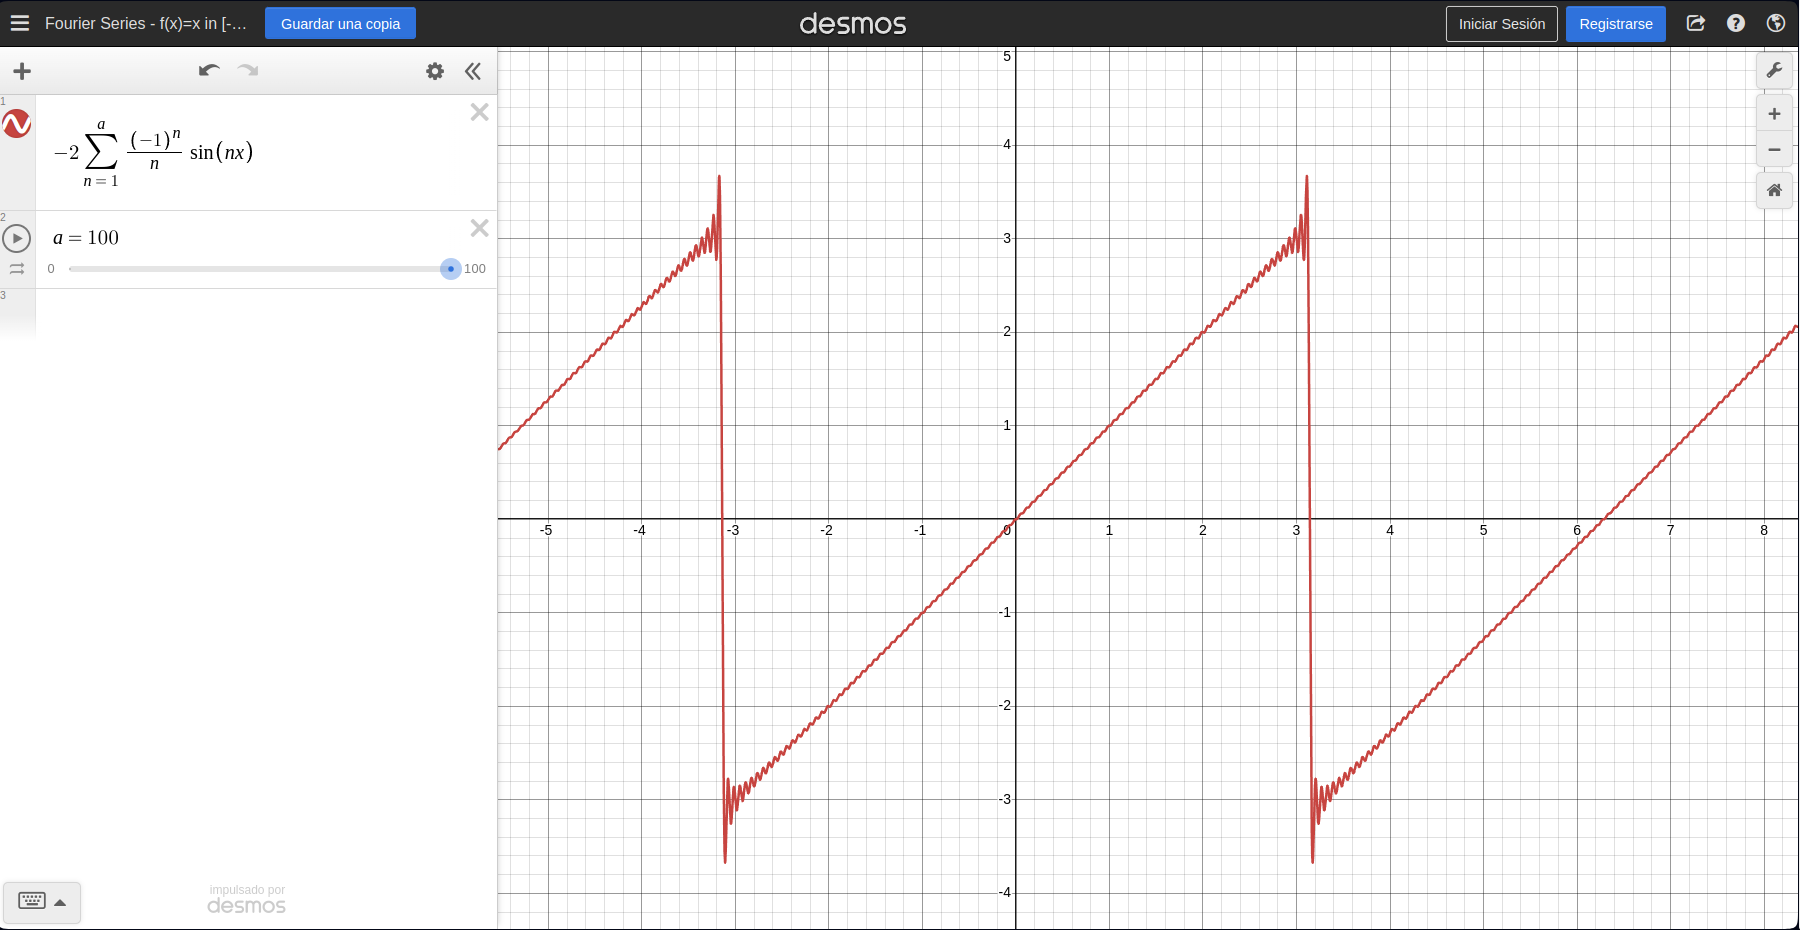
\includegraphics[width=1\textwidth]{img/chapter02/desmos-trig-series-graph.png}
	\caption{Gráfica de la serie trigonométrica de Fourier en Geogebra}
	\label{fig:desmos-trig-series}  % Etiqueta para la figura
\end{figure}
A diferencia de geogebra, la gráfica tendrá un todo un tanto más simple pero será mucho más rápida, ya que podremos hacer una serie con 100 términos y no perderá fluidez como lo haría geogebra.

\subsection{Python}
Python es un lenguaje de programación ampliamente utilizado en las aplicaciones web, el desarrollo de software, la ciencia de datos y el machine learning (ML). Los desarrolladores utilizan Python porque es eficiente y fácil de aprender, además de que se puede ejecutar en muchas plataformas diferentes. El software Python se puede descargar gratis, se integra bien a todos los tipos de sistemas y aumenta la velocidad del desarrollo ~\cite{amazonPython}.
\begin{figure}[H]
	\centering
	
\includegraphics[width=\textwidth]{img/chapter02/logo_python.png}
	\caption{Logo de Python}
	\label{fig:pythonl-ogo}  % Etiqueta para la figura
\end{figure}
La versatilidad de python permiten que se creen librerías para todo tipo de tareas con él, una de ellas es la de hacer cálculos matemáticos y creación de gráficos, de los cuales, podemos tomar funciones especificas para ayudarnos en el calculo de series de Fourier. 

\subsubsection{Sympy / Matplotlib}
SymPy y Matplotlib son dos bibliotecas de Python utilizadas en el dentro de las matemáticas y la visualización de datos. SymPy es una biblioteca de matemáticas simbólicas que permite realizar manipulaciones algebraicas, resolver ecuaciones, derivar e integrar funciones ~\cite{sympy2024}. Por otro lado, Matplotlib es una biblioteca de visualización que permite crear gráficos estáticos, interactivos y animados ~\cite{matplotlib2024}. Al combinar SymPy con Matplotlib, es posible pueden realizar cálculos simbólicos complejos y representar visualmente los resultados de manera clara y efectiva. 
\subsubsection{Prueba Python con Sympy y Matplotlib}
Para este caso, utilizaremos las funciones de integración numérica de Sympy para calcular los coeficientes de la serie trigonométrica y usando las funciones de graficación de Matplotlib, crearemos un gráfico para visualizar la función original con su aproximación de Fourier, para esto usamos el código en \hyperref[app2:complex-code-python-matplotlib-sympy]{Apendice B}. 
\begin{figure}[H]
	\centering
	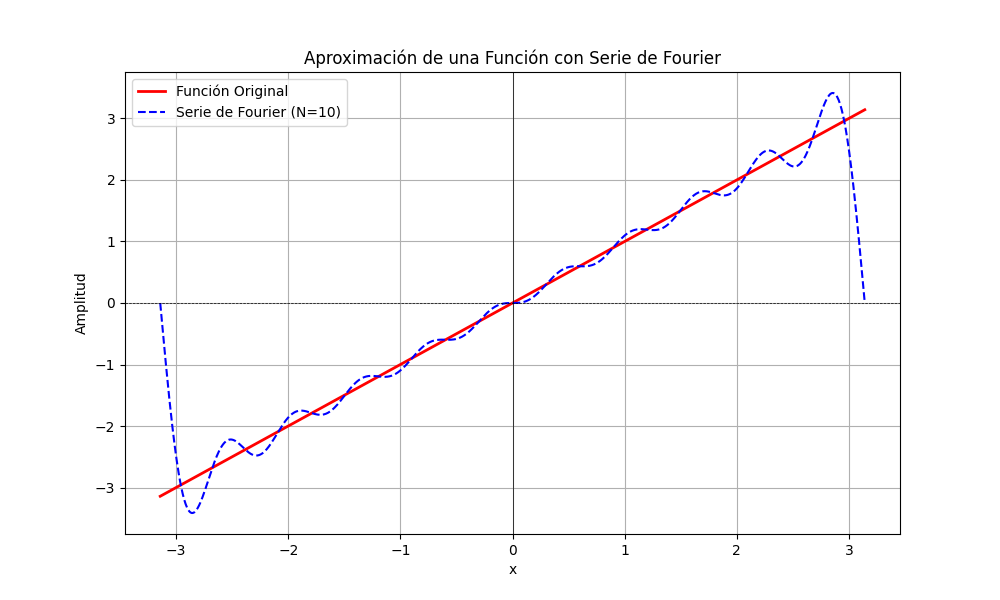
\includegraphics[width=1\textwidth]{img/chapter02/python-sympy-matplotlib.png}
	\caption{Gráfica de la serie trigonométrica y/o exponencial de Fourier en Python con Sympy y Matplotlib}
	\label{fig:python-matplotlib-sympy-trig-series}  % Etiqueta para la figura
\end{figure}
Ahora, si hacemos unos cambios en el código para que calcule el coeficiente de la serie exponencial compleja \hyperref[app2:complex-code-python-matplotlib-sympy], obtendremos exactamente la misma gráfica en \ref{fig:python-matplotlib-sympy-trig-series}, notando que Sympy es capaz de simplificar la parte imaginaria de la serie exponencial compleja para poder ver la parte real resultante en la gráfica.

\subsubsection{Manim}
Manim es una biblioteca de Python de código abierto diseñada para la creación de animaciones matemáticas de alta calidad. Desarrollada inicialmente por Grant Sanderson para su canal de YouTube "3Blue1Brown", Manim permite crear animaciones dinámicas y precisas de manera intuitiva y atractiva. La herramienta ofrece un control detallado sobre cada aspecto de la animación~\cite{Manim2024}.
\subsubsection{Prueba Python con Manim}
Para poder usar a manim, debemos definir toda la expresión de la serie trigonométrica y usar las funciones que nos ofrece manim para hacer la animación como se detalla en el código en \hyperref[app2:trig-code-python-manim]{Apendice B}.
\begin{figure}[H]
	\centering
	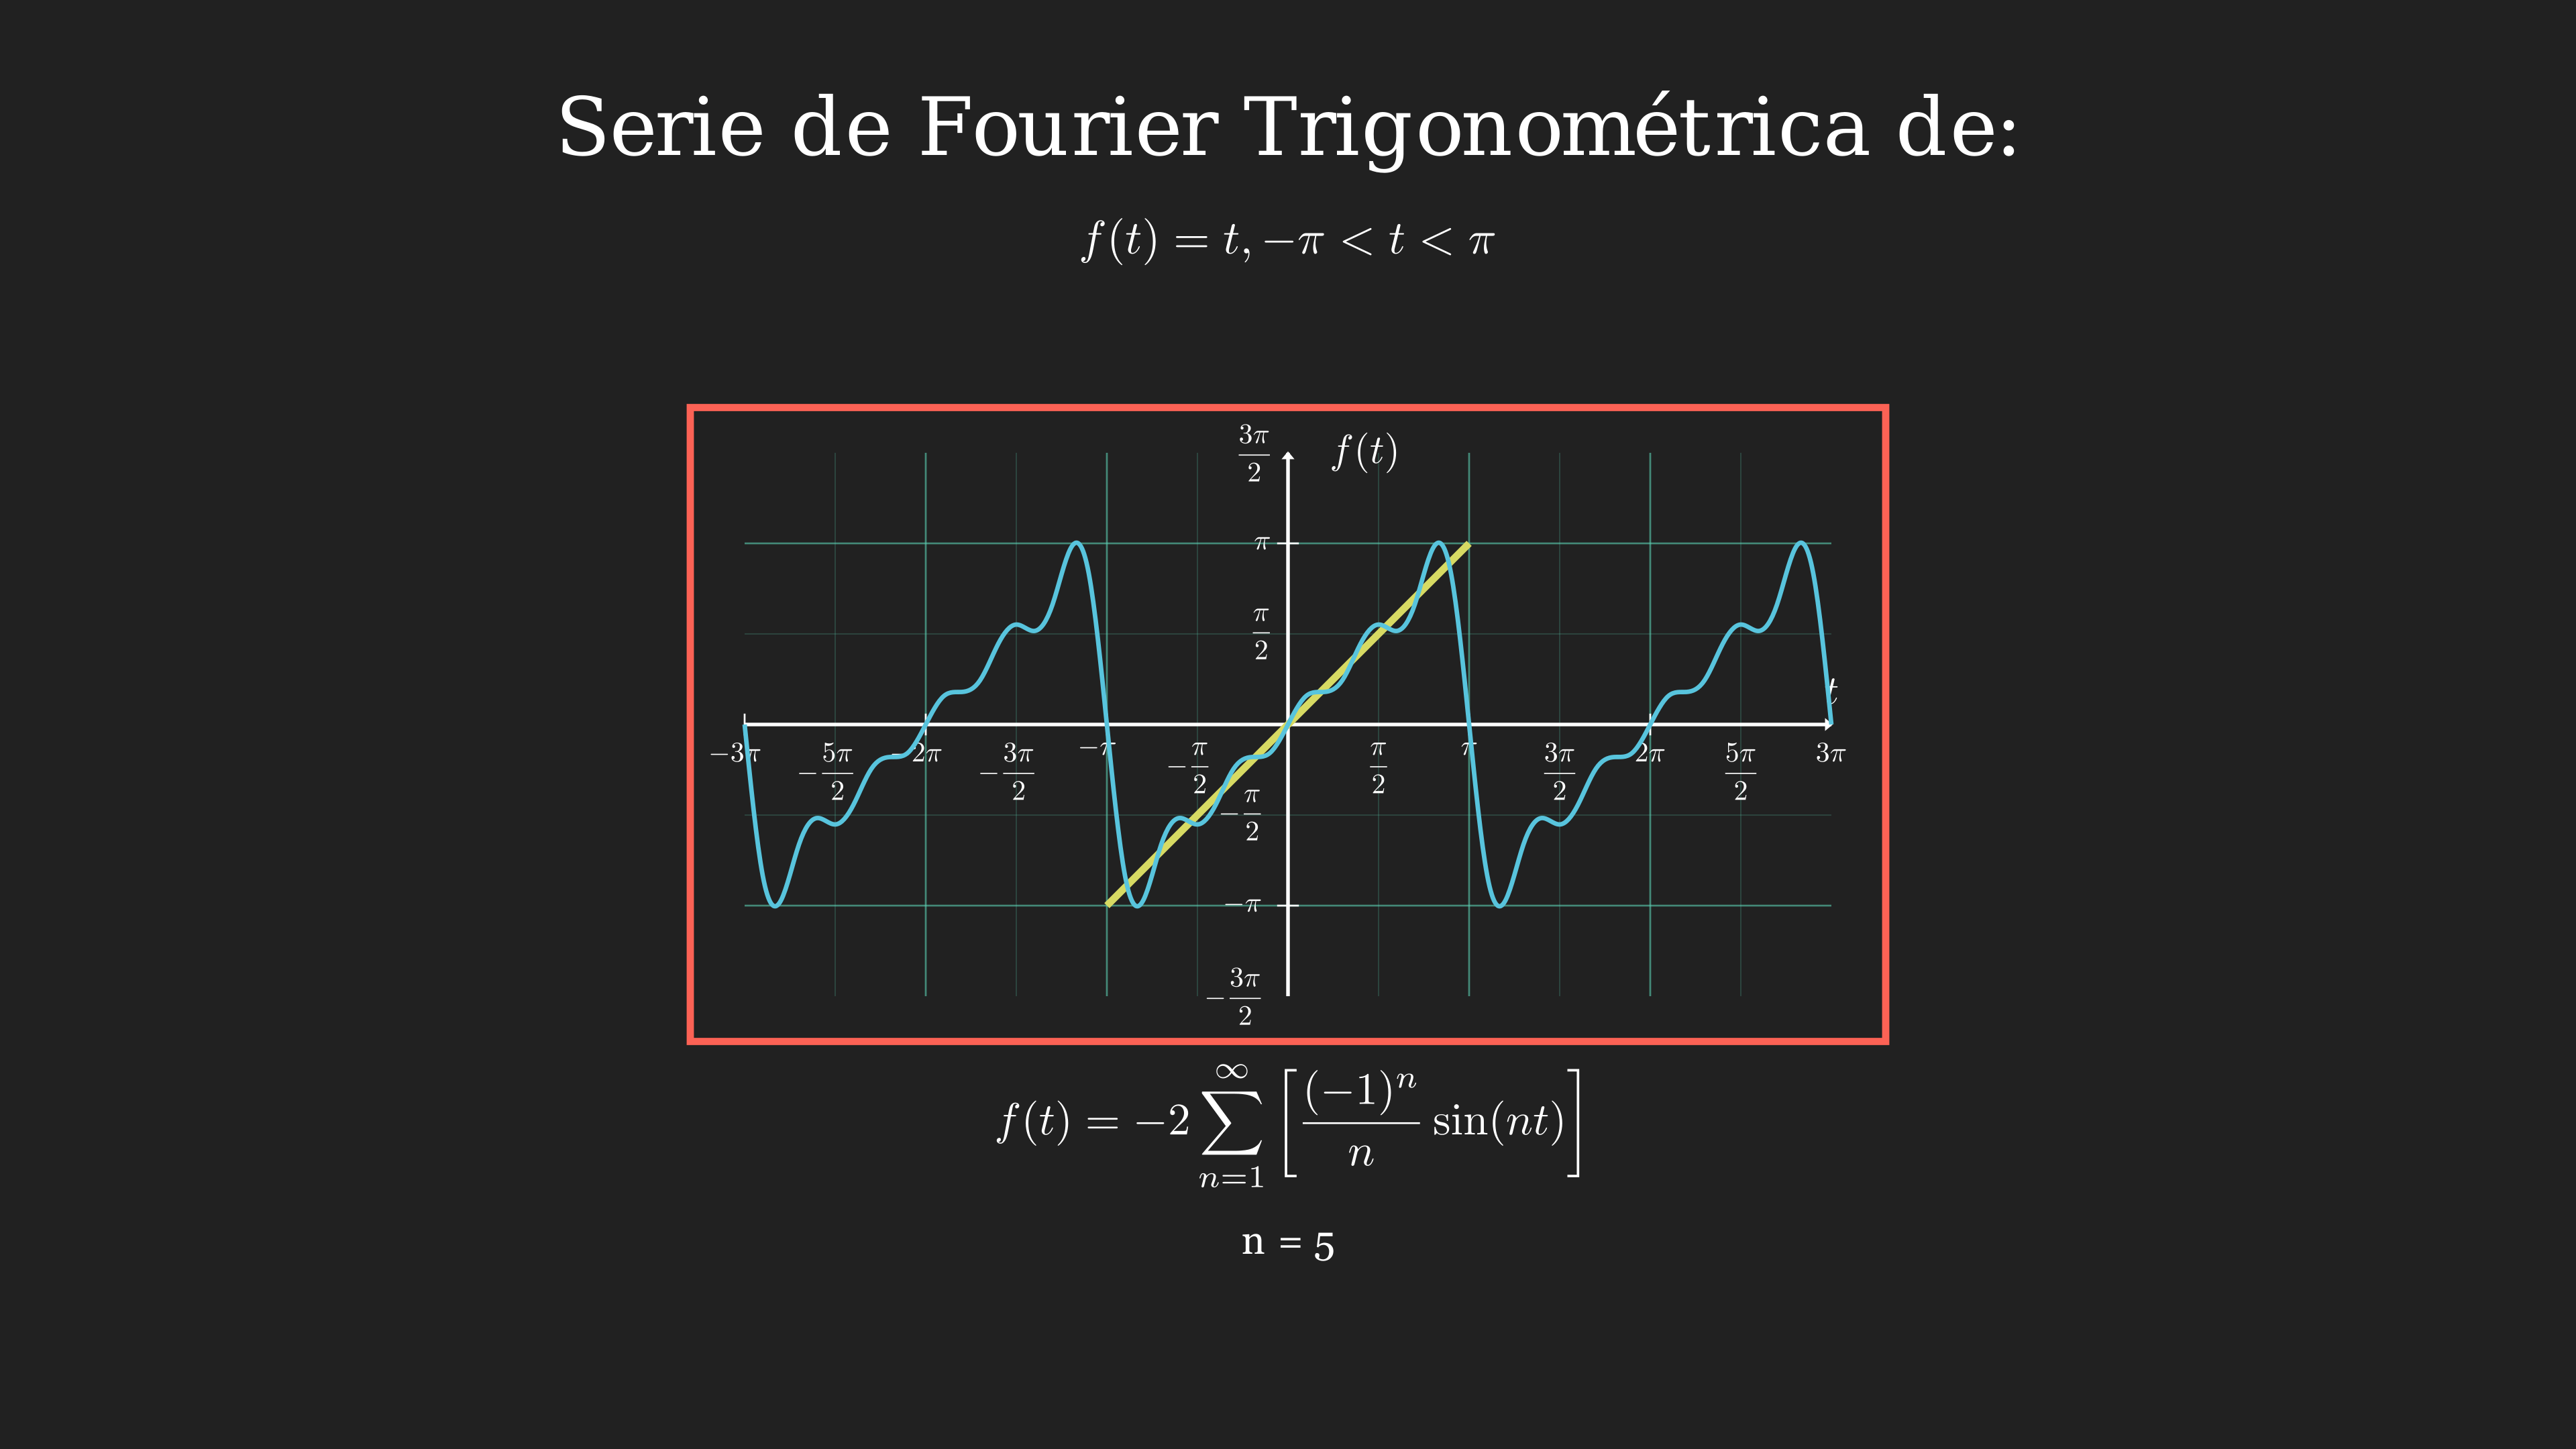
\includegraphics[width=1\textwidth]{img/chapter02/manim-trig-series-graph.png}
	\caption{Gráfica de la serie trigonométrica de Fourier en Python con Manim}
	\label{fig:python-manim-trig-series}  % Etiqueta para la figura
\end{figure}
Ahora, ejecutamos el código en \hyperref[app2:complex-code-python-manim]{Apendice B} para la serie compleja y obtenemos la siguiente salida.
\begin{figure}[H]
	\centering
	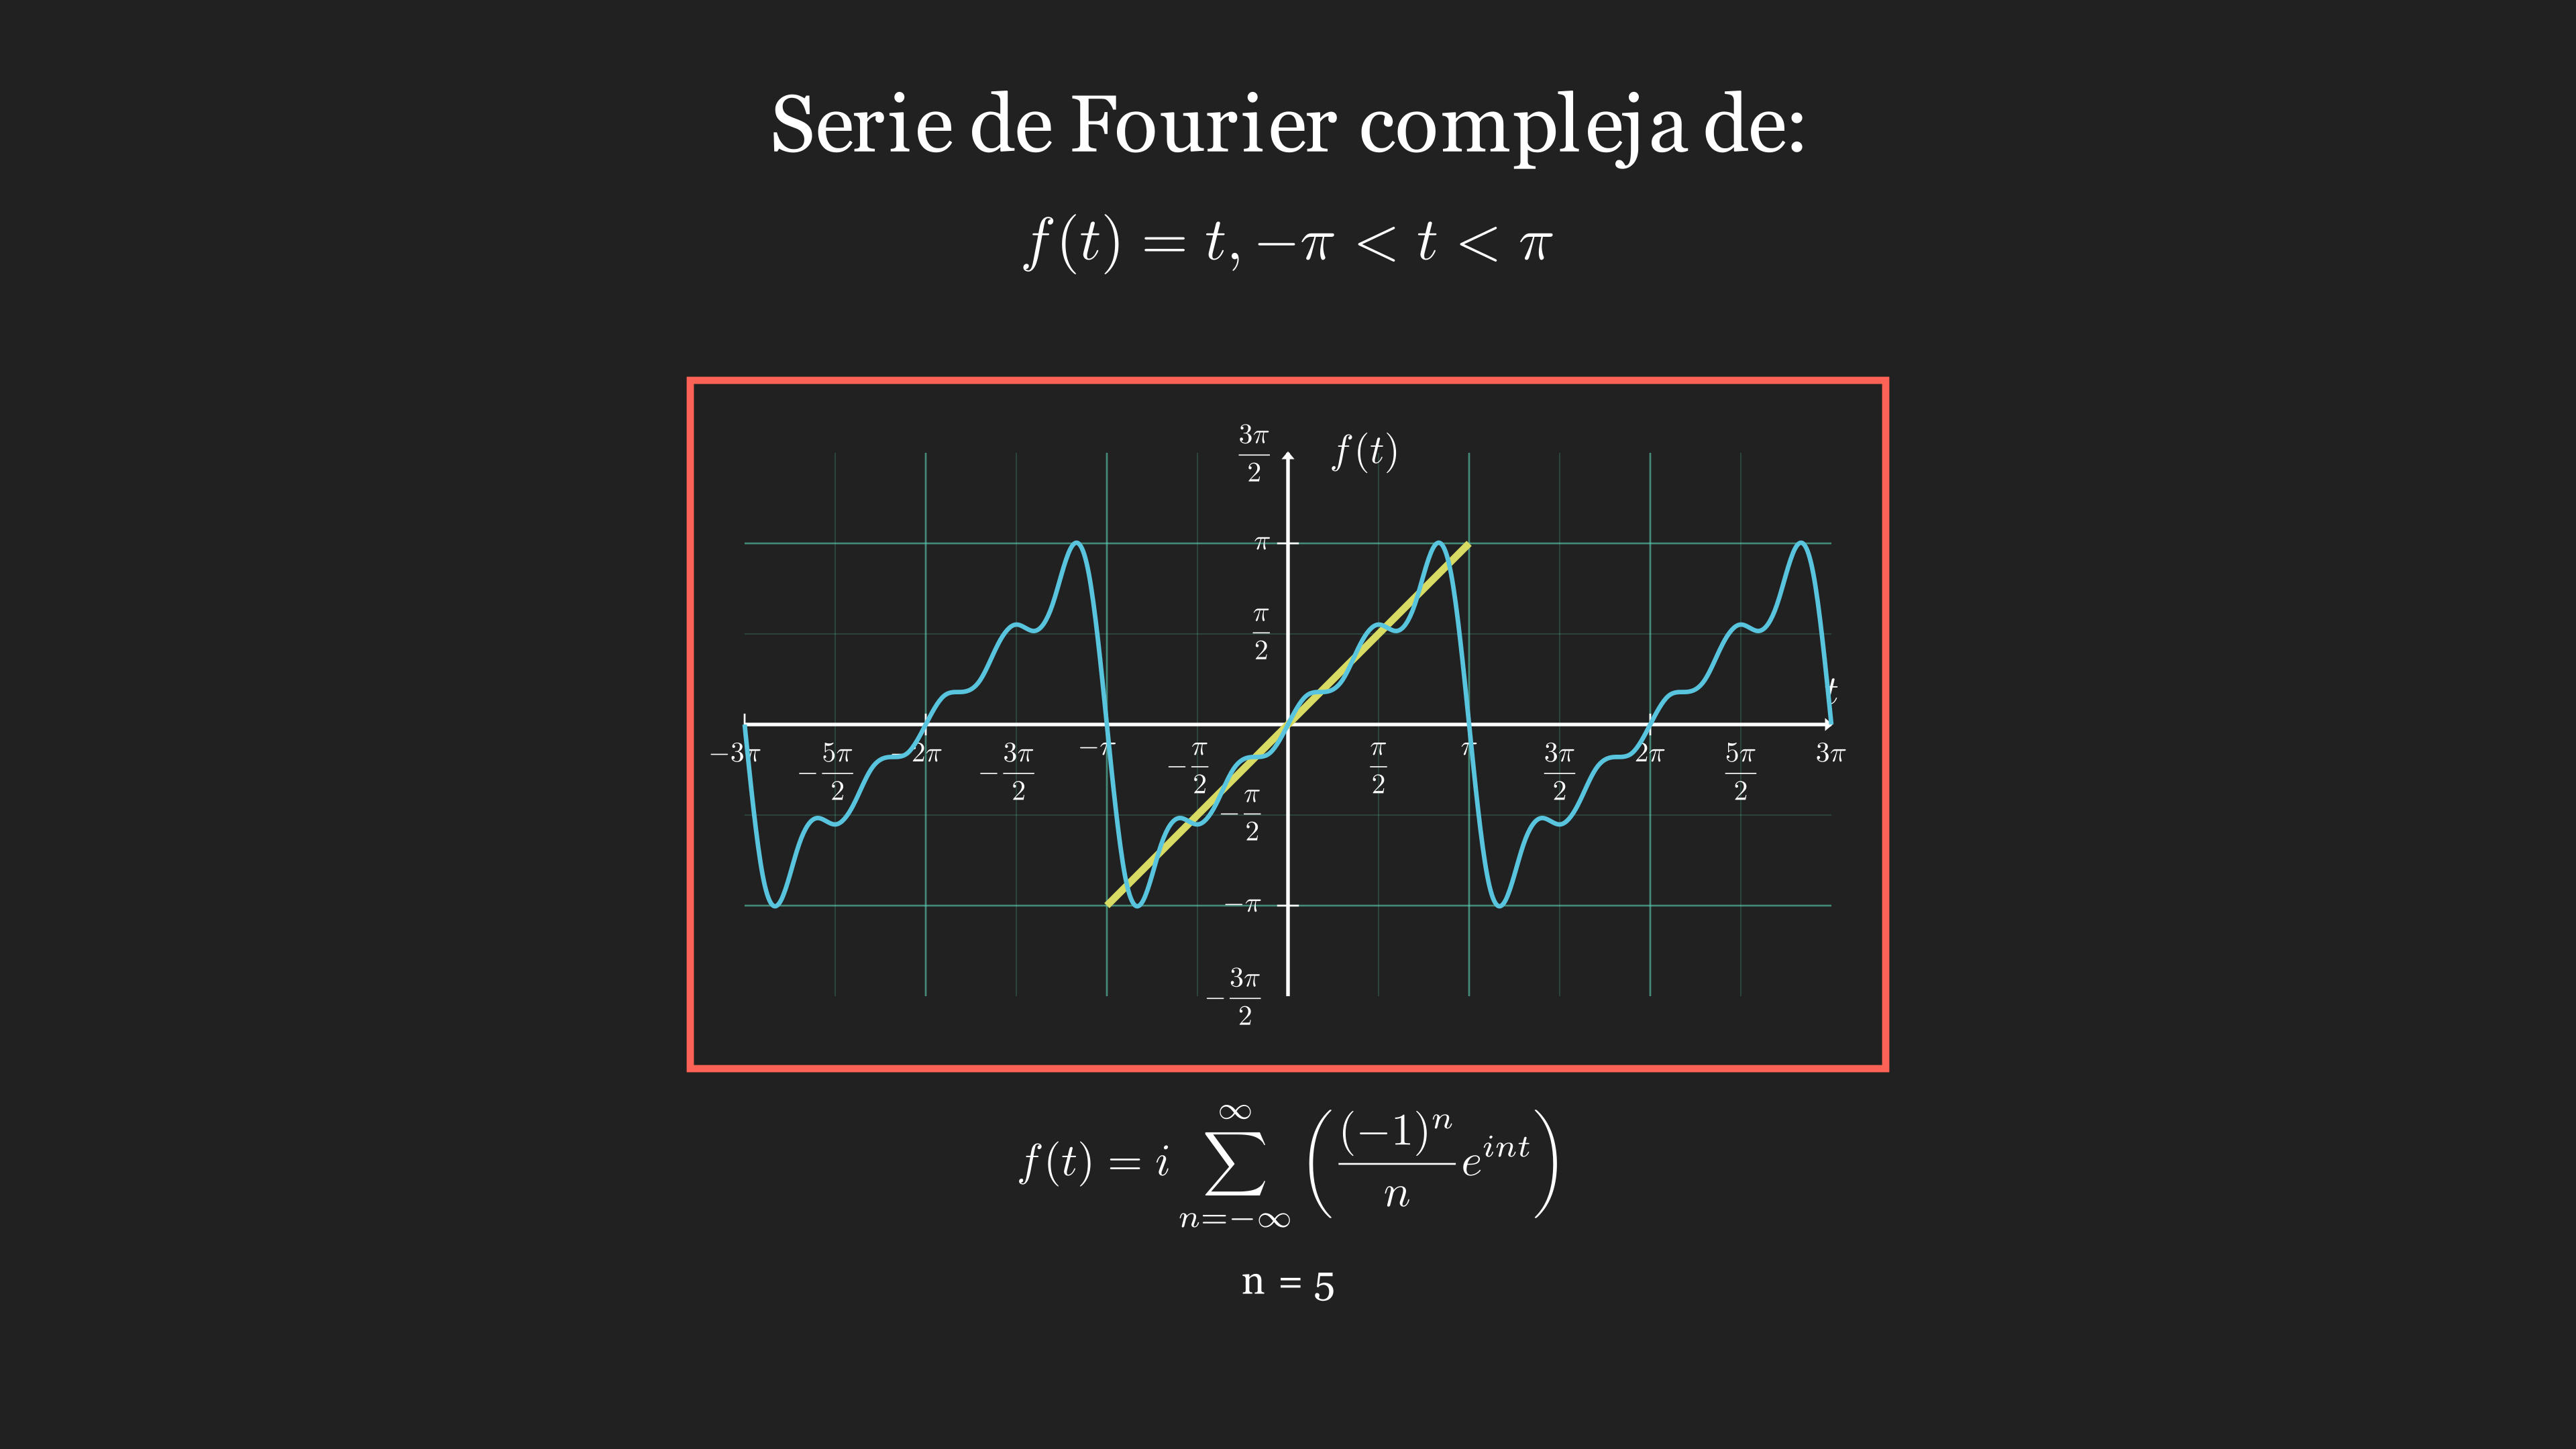
\includegraphics[width=1\textwidth]{img/chapter02/manim-complex-series-graph.png}
	\caption{Gráfica de la serie compleja de Fourier en Python con Manim}
	\label{fig:python-manim-complex-series}  % Etiqueta para la figura
\end{figure}
Manim genera gráficas impecables con animaciones fluidas y limpias, sin embargo debemos recordar que los coeficientes deben ser calculados previamente ademas de que tardará bastante tiempo en renderizar el video o imagen dependiendo de la cantidad de calculo que tenga que resolver o la calidad de la imagen.
\section{Comparativa del Funcionamiento de las Herramientas}

\begin{longtable}{ | m{2cm} | m{4cm} | m{4cm} | m{3cm} | }
	\rowcolor{black!75}
	\head {SOFTWARE} & \head {VENTAJAS} & \head {DESVENTAJAS} & \head {PRECIO} \\ \hline
	\endfirsthead
	\multicolumn{4}{c}{{\tablename\ \thetable{} -- continuación}} \\
	\rowcolor{black!75}
	\head {SOFTWARE} & \head {VENTAJAS} & \head {DESVENTAJAS} & \head {PRECIO} \\ \hline
	\endhead
	\hline \multicolumn{4}{r}{{Continúa en la siguiente página}} \\
	\endfoot
	\hline
	\endlastfoot
	Wolfram Alpha & Funciones propias para series de Fourier; Integrando, puede obtener cualquier coeficiente en su forma más simplificada. & Las funciones de series de Fourier se limitan en su periodo; Gráfica no intuitiva & Desde MXN \$1,200.00 anuales para estudiantes. \\ \hline
	Symbolab & Interfaz amigable; Función dedicada para la serie trigonométrica & Puede calcular coeficientes si integramos por aparte; No muestra gráfica & Planes básicos gratuitos; suscripción mensual para funciones avanzadas. \\ \hline
	Matlab & Potente para realizar cálculos y visualización dinámica & Requiere conocimientos previos de programación en Matlab; licencia cara para profesionales. & Desde USD\$99 anuales para estudiantes. \\ \hline
	Maple & Puede calcular cualquier coeficiente y graficar la serie trigonométrica & Interfaz limitada y menos intuitiva; Poco flexible al usarlo; Requiere conocimientos en REPL & Planes de estudiantes y profesionales, precio varía. \\ \hline
	Maxima & Permite calcular cualquier coeficiente y expandirlo en serie además de mostrar una gráfica medianamente interactiva además de ser extremadamente liviano & Interfaz limitada y menos intuitiva; no tan popular, menos soporte comunitario; Requiere conocimientos en REPL & Gratuito, de código abierto. \\ \hline
	Geogebra & Gráficas extremadamente dinámicas e interactivas; Puede graficar cualquier serie trigonométrica. & Requiere realizar calcular los coeficientes; Limitado a la serie trigonométrica.; Pesado al hacer los cálculos para graficar & Gratuito, de código abierto. \\ \hline
	Desmos & Gráficas extremadamente dinámicas e interactivas; Puede graficar cualquier serie trigonométrica; Liviano. & Requiere cálculos previos de los coeficientes; Limitado a serie trigonométrica. & Gratuito, de código abierto. \\ \hline
	Matplotlib / Sympy & Permite calcular series exponenciales y complejas, además de mostrar una gráfica medianamente interactiva & Requiere conocimientos de Python y programación avanzada; menos intuitivo para principiantes. & Gratuito, de código abierto. \\ \hline
	Manim & Puede graficar cualquier serie de Fourier mientras conozcamos sus coeficientes y expresión & Curva de aprendizaje alta; requiere conocimientos avanzados de Python y Manim; Requiere calcular la serie previamente. & Gratuito, de código abierto. \\ \hline
	\rowcolor{white}\caption{Comparación de software para cálculos matemáticos y visualización de datos} \label{tabla:Comparativa de los sitemas vistos en función de las series de Fourier} \\
\end{longtable}

De esta tabla podemos observar que si bien, hay opciones que para calculo simbólico sumamente potentes que nos permiten calcular los coeficientes, estás se ven limitadas en la visualización de generar una gráfica dinámica e intuitiva, mientras que las que ofrecen una mejor visualización de las series en las gráficas no siempre pueden hacer los cálculos o algunas no tienen forma de graficar cuando la serie presenta números complejos, sin mencionar que la mayoría requiere de conocimientos en programación especializado en el lenguaje de la herramienta.

%\section{Trabajos y Proyectos Relacionados}
%En esta sección se analizarán trabajos académicos y proyectos de investigación que han desarrollado herramientas similares o que abordan la enseñanza de series de Fourier y el uso de plataformas interactivas para la educación matemática. 

%\begin{table}[h]
%	\centering
%	\begin{tabular}{ | m{2.5cm} | m{6.5cm} | m{4cm} | }
%		\rowcolor{black!75}
%		\head {SOFTWARE} & \head {CARACTERÍSTICAS} & \head {PRECIO} \\ \hline
%		Wolfram Alpha & Potente motor de conocimiento computacional para cálculos matemáticos y gráficos. No especializado en series de Fourier.~\cite{wolfram2024}  & Desde MXN \$1,200.00 anuales para estudiantes, plan gratuito limitado. \\ \hline
%		Geogebra & Herramienta dinámica para construcciones geométricas y gráficas. Requiere cálculos previos para series de Fourier.~\cite{GeoGebra2024} & Software libre y código abierto \\ \hline
%		Desmos  & Similar a Geogebra es una calculadora gráfica en línea para cálculos y gráficos, incluida la representación de series de Fourier. Requiere cálculos previos para series de Fourier.~\cite{Desmos2024} & Software libre y código abierto\\ \hline
%		Manim & Librería de animación en Python para visualizaciones matemáticas, incluida la animación de series de Fourier. Requiere conocimientos de programación y cálculos previos.~\cite{Manim2024} & Software libre y código abierto \\ \hline
%		Matlab  & Entorno de programación para cálculos numéricos y visualización de datos, con herramientas específicas para series de Fourier. Requiere conocimientos en programación.~\cite{MathWorks2024} & Desde USD\$99 (aprox. MXN\$1627.82) anuales para estudiantes.\\ \hline
%	\end{tabular}
%	\caption{Comparación de software para cálculos matemáticos y visualización de datos}
%	\label{tabla:software}
%\end{table}
